
%%
%%
%%
%% This is the Rnw file which is used to build the static seqHMM vignette
%%
%%
%%
%%
\documentclass[12pt]{article}\usepackage[]{graphicx}\usepackage[]{color}
%% maxwidth is the original width if it is less than linewidth
%% otherwise use linewidth (to make sure the graphics do not exceed the margin)
\makeatletter
\def\maxwidth{ %
  \ifdim\Gin@nat@width>\linewidth
    \linewidth
  \else
    \Gin@nat@width
  \fi
}
\makeatother

\definecolor{fgcolor}{rgb}{0.345, 0.345, 0.345}
\newcommand{\hlnum}[1]{\textcolor[rgb]{0.686,0.059,0.569}{#1}}%
\newcommand{\hlstr}[1]{\textcolor[rgb]{0.192,0.494,0.8}{#1}}%
\newcommand{\hlcom}[1]{\textcolor[rgb]{0.678,0.584,0.686}{\textit{#1}}}%
\newcommand{\hlopt}[1]{\textcolor[rgb]{0,0,0}{#1}}%
\newcommand{\hlstd}[1]{\textcolor[rgb]{0.345,0.345,0.345}{#1}}%
\newcommand{\hlkwa}[1]{\textcolor[rgb]{0.161,0.373,0.58}{\textbf{#1}}}%
\newcommand{\hlkwb}[1]{\textcolor[rgb]{0.69,0.353,0.396}{#1}}%
\newcommand{\hlkwc}[1]{\textcolor[rgb]{0.333,0.667,0.333}{#1}}%
\newcommand{\hlkwd}[1]{\textcolor[rgb]{0.737,0.353,0.396}{\textbf{#1}}}%

\usepackage{framed}
\makeatletter
\newenvironment{kframe}{%
 \def\at@end@of@kframe{}%
 \ifinner\ifhmode%
  \def\at@end@of@kframe{\end{minipage}}%
  \begin{minipage}{\columnwidth}%
 \fi\fi%
 \def\FrameCommand##1{\hskip\@totalleftmargin \hskip-\fboxsep
 \colorbox{shadecolor}{##1}\hskip-\fboxsep
     % There is no \\@totalrightmargin, so:
     \hskip-\linewidth \hskip-\@totalleftmargin \hskip\columnwidth}%
 \MakeFramed {\advance\hsize-\width
   \@totalleftmargin\z@ \linewidth\hsize
   \@setminipage}}%
 {\par\unskip\endMakeFramed%
 \at@end@of@kframe}
\makeatother

\definecolor{shadecolor}{rgb}{.97, .97, .97}
\definecolor{messagecolor}{rgb}{0, 0, 0}
\definecolor{warningcolor}{rgb}{1, 0, 1}
\definecolor{errorcolor}{rgb}{1, 0, 0}
\newenvironment{knitrout}{}{} % an empty environment to be redefined in TeX

\usepackage{alltt}
\usepackage[sc]{mathpazo}
\usepackage{textcomp} %for oms warning on linux
\usepackage{amsmath}
\usepackage{graphicx,psfrag,epsf}
\usepackage{enumerate}
\usepackage{natbib}
\usepackage{url} % not crucial - just used below for the URL
\usepackage{makeidx}
\usepackage[nottoc]{tocbibind}
\usepackage{hyperref}
\hypersetup{
    colorlinks=true, % set true if you want colored links
    linktoc=all,     % set to all if you want both sections and subsections linked
    linkcolor=black,  % choose some color if you want links to stand out
    citecolor=black,
    urlcolor=black
}


\addtolength{\oddsidemargin}{-.5in}%
\addtolength{\evensidemargin}{-.5in}%
\addtolength{\textwidth}{1in}%
\addtolength{\textheight}{1.3in}%
\addtolength{\topmargin}{-.8in}%

\setcounter{tocdepth}{2}

\makeindex
\IfFileExists{upquote.sty}{\usepackage{upquote}}{}
\begin{document}


\def\spacingset#1{\renewcommand{\baselinestretch}%
{#1}\small\normalsize} \spacingset{1}



  \title{\bf Using the \texttt{seqHMM} package \\
  for mixture hidden Markov models \\
  \large (Version 1.0)}
  \author{Satu Helske
    and
    Jouni Helske \\
    Department of Mathematics and Statistics, University of Jyv{\"a}skyl{\"a}, Finland}




\maketitle

\tableofcontents

\bigskip

\spacingset{1.45}

\section{Introduction}

This vignette is supplementary material to the paper by \citet{HelskeHelske}. It shows more detailed examples on how to use features of the \texttt{seqHMM} package in R \citep{RCoreTeam2015}. The package is designed for fitting hidden (or latent) Markov models (HMMs) and mixture hidden Markov models (MHMMs) for social sequence data and other categorical time series. It supports models for one or multiple subjects with one or multiple interdependent sequences (channels). External covariates can be added to explain cluster membership in MHMMs. The \texttt{seqHMM} package provides functions for evaluating and comparing models, as well as functions for easy plotting of multichannel sequences and hidden Markov models. Other restricted variants of the MHMM can also be estimated, e.g. latent class models, binomial and multinomial regression models, Markov models, and mixture Markov models.

Package is written mostly in C++, and it supports parallel processing via OpenMP. For improved numerical accuracy, the recursive algoritms can be computed in log-space, which reduces under- and overflow problems in forward--backward algorithm even more than classical scaling approach (which is still a default option in \texttt{seqHMM} as log-space approach is computationally less efficient).

We start by showing how the package is installed and then prepare the example data before illustrating features of the package. We try to cover a wide range of examples to show different ways of using the functions. More examples and information are available in the documentation of the function (or data) by typing \texttt{?function\_name} or equivalently \texttt{help(function\_name)}.


\section{Installation}

The seqHMM package is currently available in Github:
  \url{https://github.com/helske/seqHMM}.
It can be easily installed in R via the \texttt{devtools} package by writing the following lines in R.

\begin{knitrout}
\definecolor{shadecolor}{rgb}{0.969, 0.969, 0.969}\color{fgcolor}\begin{kframe}
\begin{alltt}
\hlkwd{install.packages}\hlstd{(}\hlstr{"devtools"}\hlstd{)}
\hlkwd{library}\hlstd{(devtools)}
\hlkwd{install_github}\hlstd{(}\hlstr{"helske/seqHMM"}\hlstd{)}
\end{alltt}
\end{kframe}
\end{knitrout}
After the installation (only needed the first time) the package is loaded with the \texttt{library} function.

\begin{knitrout}
\definecolor{shadecolor}{rgb}{0.969, 0.969, 0.969}\color{fgcolor}\begin{kframe}
\begin{alltt}
\hlkwd{library}\hlstd{(seqHMM)}
\end{alltt}
\end{kframe}
\end{knitrout}

\section{Example data}
\label{sec:data}

The example data \texttt{biofam}\index{biofam@\texttt{biofam}} comes with the \texttt{TraMineR} package \citep{Gabadinho2011} which is installed automatically with the \texttt{seqHMM} package. It is a sample of 2000 individuals born in 1909--1972, constructed from the Swiss Household Panel survey in 2002. The data set contains sequences of family life states from age 15 to 30 (in columns 10 to 25) and a series of covariates.

The states numbered from 0 to 7 are defined from the combination of five basic states, namely living with parents (parents), left home (left), married (marr), having children (child), and divorced: \\

\noindent
0 = "parents" \\
1 = "left" \\
2 = "married" \\
3 = "left+marr" \\
4 = "child" \\
5 = "left+child" \\
6 = "left+marr+child" \\
7 = "divorced". \\

For \texttt{seqHMM} functions, the data needs to be given as an \texttt{stslist} object. Such state sequence object is created with the \texttt{seqdef} function from the \texttt{TraMineR} package. It has attributes such as color palette and alphabet, and it also has specific methods for plotting, summarizing, and printing.

We use two versions of the same data; one with the original single-channel sequences and another version, where the same data is converted into a multichannel version.

\subsection{Single-channel data}

We start by showing a glimpse of the original sequence data (in columns 10--25) and then create a state sequence object. We set the start at age 15 and give labels to states.

\begin{knitrout}
\definecolor{shadecolor}{rgb}{0.969, 0.969, 0.969}\color{fgcolor}\begin{kframe}
\begin{alltt}
\hlkwd{data}\hlstd{(}\hlstr{"biofam"}\hlstd{,} \hlkwc{package} \hlstd{=} \hlstr{"TraMineR"}\hlstd{)}

\hlkwd{head}\hlstd{(biofam[,} \hlnum{10}\hlopt{:}\hlnum{25}\hlstd{])}
\end{alltt}
\begin{verbatim}
##      a15 a16 a17 a18 a19 a20 a21 a22 a23 a24 a25 a26 a27 a28 a29 a30
## 1167   0   0   0   0   0   0   0   0   0   3   6   6   6   6   6   6
## 514    0   1   1   1   1   1   1   1   1   1   1   3   6   6   6   6
## 1013   0   0   0   0   0   0   0   1   1   1   1   1   3   6   6   6
## 275    0   0   0   0   0   1   1   1   1   1   1   1   1   1   1   1
## 2580   0   0   0   0   0   1   1   1   1   1   1   1   1   6   6   6
## 773    0   0   0   0   0   0   0   0   0   0   0   0   0   0   0   0
\end{verbatim}
\begin{alltt}
\hlstd{biofam.seq} \hlkwb{<-} \hlkwd{seqdef}\hlstd{(}
  \hlstd{biofam[,} \hlnum{10}\hlopt{:}\hlnum{25}\hlstd{],} \hlkwc{start} \hlstd{=} \hlnum{15}\hlstd{,}
  \hlkwc{labels} \hlstd{=} \hlkwd{c}\hlstd{(}\hlstr{"parent"}\hlstd{,} \hlstr{"left"}\hlstd{,} \hlstr{"married"}\hlstd{,} \hlstr{"left+marr"}\hlstd{,} \hlstr{"child"}\hlstd{,}
             \hlstr{"left+child"}\hlstd{,} \hlstr{"left+marr+child"}\hlstd{,} \hlstr{"divorced"}\hlstd{))}
\end{alltt}
\end{kframe}
\end{knitrout}

\subsection{Multichannel data}
For showing a more complex example with multichannel sequence data, we provide an R file which creates three separate sequences from the \texttt{biofam} data. The \texttt{biofam3c} object includes a list with three sequence data sets and a data frame with covariates. Note that the divorced state in the original data does not give information on children on residence, so the those are determined according to the preceeding states.

\begin{knitrout}
\definecolor{shadecolor}{rgb}{0.969, 0.969, 0.969}\color{fgcolor}\begin{kframe}
\begin{alltt}
\hlkwd{data}\hlstd{(}\hlstr{"biofam3c"}\hlstd{)}

\hlstd{marr_seq} \hlkwb{<-} \hlkwd{seqdef}\hlstd{(biofam3c}\hlopt{$}\hlstd{married,} \hlkwc{start} \hlstd{=} \hlnum{15}\hlstd{,}
                   \hlkwc{alphabet} \hlstd{=} \hlkwd{c}\hlstd{(}\hlstr{"single"}\hlstd{,} \hlstr{"married"}\hlstd{,} \hlstr{"divorced"}\hlstd{))}
\hlstd{child_seq} \hlkwb{<-} \hlkwd{seqdef}\hlstd{(biofam3c}\hlopt{$}\hlstd{children,} \hlkwc{start} \hlstd{=} \hlnum{15}\hlstd{,}
                    \hlkwc{alphabet} \hlstd{=} \hlkwd{c}\hlstd{(}\hlstr{"childless"}\hlstd{,} \hlstr{"children"}\hlstd{))}
\hlstd{left_seq} \hlkwb{<-} \hlkwd{seqdef}\hlstd{(biofam3c}\hlopt{$}\hlstd{left,} \hlkwc{start} \hlstd{=} \hlnum{15}\hlstd{,}
                   \hlkwc{alphabet} \hlstd{=} \hlkwd{c}\hlstd{(}\hlstr{"with parents"}\hlstd{,} \hlstr{"left home"}\hlstd{))}
\end{alltt}
\end{kframe}
\end{knitrout}

\section{Plotting multichannel sequence data}

The \texttt{TraMineR} package provides several plotting options for simple single-channel sequence data with the \texttt{seqplot} function, but there are no easy options for plotting multichannel data. In \texttt{seqHMM}, such data can be plotted in several ways. We start by choosing colors for the observed states in each channel.

\begin{knitrout}
\definecolor{shadecolor}{rgb}{0.969, 0.969, 0.969}\color{fgcolor}\begin{kframe}
\begin{alltt}
\hlkwd{attr}\hlstd{(marr_seq,} \hlstr{"cpal"}\hlstd{)} \hlkwb{<-} \hlkwd{c}\hlstd{(}\hlstr{"violetred2"}\hlstd{,} \hlstr{"darkgoldenrod2"}\hlstd{,} \hlstr{"darkmagenta"}\hlstd{)}
\hlkwd{attr}\hlstd{(child_seq,} \hlstr{"cpal"}\hlstd{)} \hlkwb{<-} \hlkwd{c}\hlstd{(}\hlstr{"darkseagreen1"}\hlstd{,} \hlstr{"coral3"}\hlstd{)}
\hlkwd{attr}\hlstd{(left_seq,} \hlstr{"cpal"}\hlstd{)} \hlkwb{<-} \hlkwd{c}\hlstd{(}\hlstr{"lightblue"}\hlstd{,} \hlstr{"red3"}\hlstd{)}
\end{alltt}
\end{kframe}
\end{knitrout}

\subsection{Stacked sequence plots}

First we plot annual state distributions with the \texttt{ssplot}\index{ssplot@\texttt{ssplot}} function (ssp for Stacked Sequence Plot). The \texttt{ssplot} function accepts two types of sequence plots available in the \texttt{seqplot} function from \texttt{TraMineR}: argument \texttt{type = "d"} gives state distributions and \texttt{type = "I"} shows sequence index plots. If the list objects are given a name, those are printed as labels; otherwise the number of the channel is plotted as a label. Another option is to use the \texttt{ylab} argument to change the labels. The number of sequences is automatically printed unless either the \texttt{title} or the \texttt{title.n} argument is set to \texttt{FALSE}. Figure \ref{fig:plotd} shows the default plot for three-channel data.

\begin{knitrout}
\definecolor{shadecolor}{rgb}{0.969, 0.969, 0.969}\color{fgcolor}\begin{kframe}
\begin{alltt}
\hlkwd{ssplot}\hlstd{(}\hlkwd{list}\hlstd{(}\hlstr{"Marriage"} \hlstd{= marr_seq,} \hlstr{"Parenthood"} \hlstd{= child_seq,}
       \hlstr{"Residence"} \hlstd{= left_seq))}
\end{alltt}
\end{kframe}\begin{figure}

{\centering 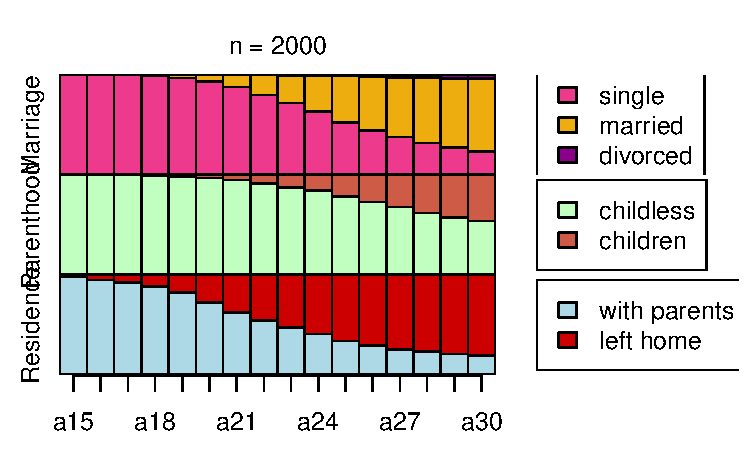
\includegraphics[width=\maxwidth]{figure/plotd-1} 

}

\caption[State distribution plots for multichannel data drawn with the \texttt{ssplot} function]{State distribution plots for multichannel data drawn with the \texttt{ssplot} function.}\label{fig:plotd}
\end{figure}


\end{knitrout}

Another option is to define function arguments with the \texttt{ssp} function\index{ssp@\texttt{ssp}} and then use previously saved arguments for plotting with a simple \texttt{plot}\index{plot.ssp@\texttt{plot.ssp}} method. In figure \ref{fig:plotI} sequences are sorted according to the beginning of the marriage sequence (the first channel). Legends are omitted from the plot. The \texttt{ylab.pos} defines the positions of the channel labels.

\begin{knitrout}
\definecolor{shadecolor}{rgb}{0.969, 0.969, 0.969}\color{fgcolor}\begin{kframe}
\begin{alltt}
\hlstd{ssp2} \hlkwb{<-} \hlkwd{ssp}\hlstd{(}
  \hlkwd{list}\hlstd{(marr_seq, child_seq, left_seq),}
  \hlkwc{type} \hlstd{=} \hlstr{"I"}\hlstd{,}\hlkwc{title} \hlstd{=} \hlstr{"Sequence index plots"}\hlstd{,}
  \hlkwc{sortv} \hlstd{=} \hlstr{"from.start"}\hlstd{,} \hlkwc{sort.channel} \hlstd{=} \hlnum{1}\hlstd{,}
  \hlkwc{withlegend} \hlstd{=} \hlnum{FALSE}\hlstd{,} \hlkwc{ylab.pos} \hlstd{=} \hlkwd{c}\hlstd{(}\hlnum{1}\hlstd{,} \hlnum{1.5}\hlstd{,} \hlnum{1}\hlstd{),}
  \hlkwc{ylab} \hlstd{=} \hlkwd{c}\hlstd{(}\hlstr{"Marriage"}\hlstd{,} \hlstr{"Parenthood"}\hlstd{,} \hlstr{"Residence"}\hlstd{))}
\hlkwd{plot}\hlstd{(ssp2)}
\end{alltt}
\end{kframe}\begin{figure}

{\centering 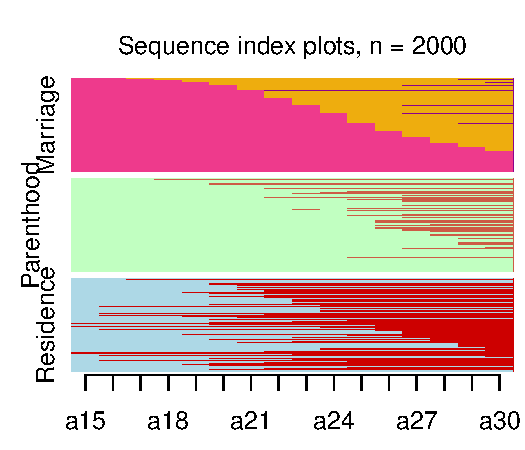
\includegraphics[width=\maxwidth]{figure/plotI-1} 

}

\caption[Sequence index plots for multichannel data defined with the \texttt{ssp} function and plotted with the \texttt{plot} method]{Sequence index plots for multichannel data defined with the \texttt{ssp} function and plotted with the \texttt{plot} method.}\label{fig:plotI}
\end{figure}


\end{knitrout}

\subsection{Plotting sequence data in a grid}

We can also plot several \texttt{ssp}\index{ssp@\texttt{ssp}} objects together. At first we define each \texttt{ssp} plot and then use the \texttt{gridplot}\index{gridplot@\texttt{gridplot}} function to arrange them in a grid. Here we plot state distributions and sequence plots for women and men in a grid with two columns and three rows, of which the bottom row is reserved for the legends. The number of rows and/or columns is determined automatically, if one or both are omitted from the call. The plots are positioned column-wise by default, but here we change to row-wise plotting order.

We start by defining the first plot, state distributions for women. We remove borders from the bars, and omit legends and the number of sequences from the title. The other plots are easy to define with the \texttt{update} function -- the user only needs to type the arguments that are different to the first call.

\begin{knitrout}
\definecolor{shadecolor}{rgb}{0.969, 0.969, 0.969}\color{fgcolor}\begin{kframe}
\begin{alltt}
\hlcom{# Preparing plots for women's state distributions}
\hlstd{ssp_f_d} \hlkwb{<-} \hlkwd{ssp}\hlstd{(}
  \hlkwc{x} \hlstd{=} \hlkwd{list}\hlstd{(marr_seq[biofam}\hlopt{$}\hlstd{sex} \hlopt{==} \hlstr{"woman"}\hlstd{,],}
           \hlstd{child_seq[biofam}\hlopt{$}\hlstd{sex} \hlopt{==} \hlstr{"woman"}\hlstd{,],}
           \hlstd{left_seq[biofam}\hlopt{$}\hlstd{sex} \hlopt{==} \hlstr{"woman"}\hlstd{,]),}
  \hlkwc{plots} \hlstd{=} \hlstr{"obs"}\hlstd{,} \hlkwc{type} \hlstd{=} \hlstr{"d"}\hlstd{,} \hlkwc{border} \hlstd{=} \hlnum{NA}\hlstd{,} \hlkwc{withlegend} \hlstd{=} \hlnum{FALSE}\hlstd{,}
  \hlkwc{title} \hlstd{=} \hlstr{"State distributions for women"}\hlstd{,} \hlkwc{title.n} \hlstd{=} \hlnum{FALSE}\hlstd{,}
  \hlkwc{ylab} \hlstd{=} \hlkwd{c}\hlstd{(}\hlstr{"Marriage"}\hlstd{,} \hlstr{"Parenthood"}\hlstd{,} \hlstr{"Residence"}\hlstd{),}
  \hlkwc{xlab} \hlstd{=} \hlstr{"Age"}\hlstd{,} \hlkwc{xtlab} \hlstd{=} \hlnum{15}\hlopt{:}\hlnum{30}\hlstd{)}

\hlcom{# Same plot, but sequences instead of state distributions}
\hlstd{ssp_f_I} \hlkwb{<-} \hlkwd{update}\hlstd{(}
  \hlstd{ssp_f_d,} \hlkwc{type} \hlstd{=} \hlstr{"I"}\hlstd{,} \hlkwc{sortv} \hlstd{=} \hlstr{"mds.obs"}\hlstd{,}
  \hlkwc{title} \hlstd{=} \hlstr{"Sequences for women"}\hlstd{,} \hlkwc{title.n} \hlstd{=} \hlnum{TRUE}\hlstd{)}

\hlcom{# State distributions with men's data}
\hlstd{ssp_m_d} \hlkwb{<-} \hlkwd{update}\hlstd{(}
  \hlstd{ssp_f_d,} \hlkwc{title} \hlstd{=} \hlstr{"State distributions for men"}\hlstd{,}
  \hlkwc{x} \hlstd{=} \hlkwd{list}\hlstd{(marr_seq[biofam}\hlopt{$}\hlstd{sex} \hlopt{==} \hlstr{"man"}\hlstd{,],}
           \hlstd{child_seq[biofam}\hlopt{$}\hlstd{sex} \hlopt{==} \hlstr{"man"}\hlstd{,],}
           \hlstd{left_seq[biofam}\hlopt{$}\hlstd{sex} \hlopt{==} \hlstr{"man"}\hlstd{,]))}

\hlcom{# Men's sequences}
\hlstd{ssp_m_I} \hlkwb{<-} \hlkwd{update}\hlstd{(}
  \hlstd{ssp_m_d,} \hlkwc{type} \hlstd{=} \hlstr{"I"}\hlstd{,} \hlkwc{sortv} \hlstd{=} \hlstr{"mds.obs"}\hlstd{,}
  \hlkwc{title} \hlstd{=} \hlstr{"Sequences for men"}\hlstd{,} \hlkwc{title.n} \hlstd{=} \hlnum{TRUE}\hlstd{)}

\hlkwd{gridplot}\hlstd{(}
  \hlkwd{list}\hlstd{(ssp_f_d, ssp_f_I, ssp_m_d, ssp_m_I),} \hlkwc{ncol} \hlstd{=} \hlnum{2}\hlstd{,}
  \hlkwc{byrow} \hlstd{=} \hlnum{TRUE}\hlstd{,} \hlkwc{row.prop}\hlstd{=}\hlkwd{c}\hlstd{(}\hlnum{0.42}\hlstd{,} \hlnum{0.42}\hlstd{,} \hlnum{0.16}\hlstd{))}
\end{alltt}
\end{kframe}\begin{figure}

{\centering 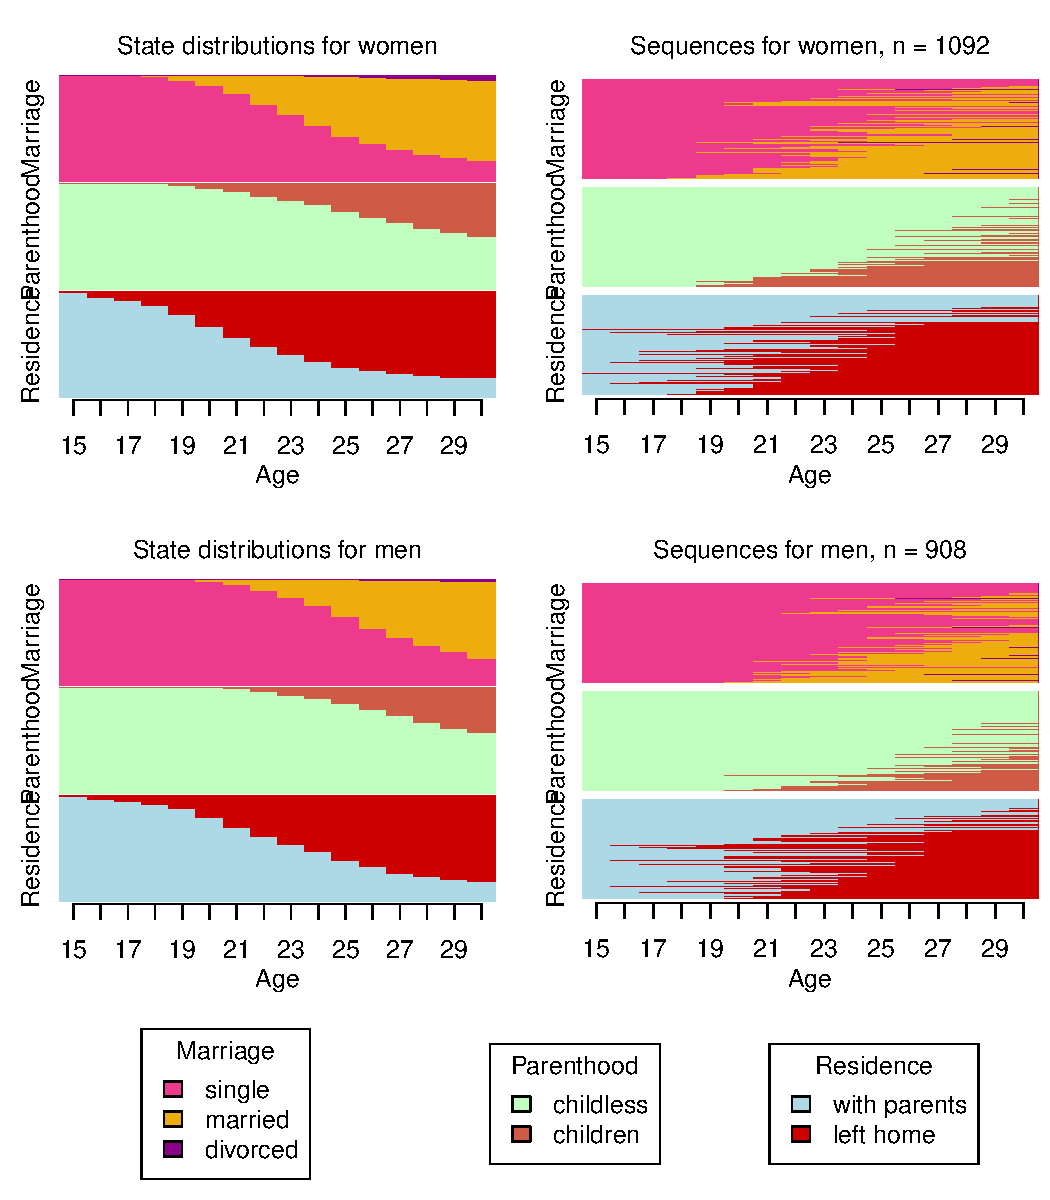
\includegraphics[width=\maxwidth]{figure/gridplotfm2-1} 

}

\caption[Plotting several \texttt{ssp} plots in a grid with the \texttt{gridplot} function]{Plotting several \texttt{ssp} plots in a grid with the \texttt{gridplot} function.}\label{fig:gridplotfm2}
\end{figure}


\end{knitrout}


The \texttt{gridplot} function is able to create legends automatically using the states given in the first \texttt{ssp} object. If the objects contain different data with different states, legends can be included in the \texttt{ssp} objects and omitted from the \texttt{gridplot}. Figure \ref{fig:gridplot2} illustrates such plot using both the original \texttt{biofam} data and the three-channel version.

\begin{knitrout}
\definecolor{shadecolor}{rgb}{0.969, 0.969, 0.969}\color{fgcolor}\begin{kframe}
\begin{alltt}
\hlstd{ssp_d} \hlkwb{<-} \hlkwd{ssp}\hlstd{(}
  \hlstd{biofam.seq,} \hlkwc{border} \hlstd{=} \hlnum{NA}\hlstd{,} \hlkwc{title.n} \hlstd{=} \hlnum{FALSE}\hlstd{,}
  \hlkwc{title} \hlstd{=} \hlstr{"State distributions (original states)"}\hlstd{,}
  \hlkwc{yaxis} \hlstd{=} \hlnum{TRUE}\hlstd{,} \hlkwc{ylab} \hlstd{=} \hlnum{FALSE}\hlstd{,}
  \hlkwc{withlegend} \hlstd{=} \hlstr{"bottom"}\hlstd{,} \hlkwc{ncol.legend} \hlstd{=} \hlnum{2}\hlstd{)}

\hlstd{ssp_I} \hlkwb{<-} \hlkwd{ssp}\hlstd{(}
  \hlkwd{list}\hlstd{(}\hlstr{"Marriage"} \hlstd{= marr_seq,} \hlstr{"Parenthood"} \hlstd{= child_seq,}
       \hlstr{"Residence"} \hlstd{= left_seq),}
  \hlkwc{type} \hlstd{=} \hlstr{"I"}\hlstd{,} \hlkwc{sortv} \hlstd{=} \hlstr{"from.end"}\hlstd{,} \hlkwc{title} \hlstd{=} \hlstr{"Sequences"}\hlstd{,}
  \hlkwc{xaxis} \hlstd{=} \hlnum{FALSE}\hlstd{,} \hlkwc{legend.prop} \hlstd{=} \hlnum{0.5}\hlstd{)}

\hlkwd{gridplot}\hlstd{(}
  \hlkwd{list}\hlstd{(ssp_d, ssp_I),} \hlkwc{ncol} \hlstd{=} \hlnum{2}\hlstd{,} \hlkwc{withlegend} \hlstd{=} \hlnum{FALSE}\hlstd{,} \hlkwc{col.prop} \hlstd{=} \hlkwd{c}\hlstd{(}\hlnum{0.5}\hlstd{,} \hlnum{0.5}\hlstd{))}
\end{alltt}
\end{kframe}\begin{figure}

{\centering 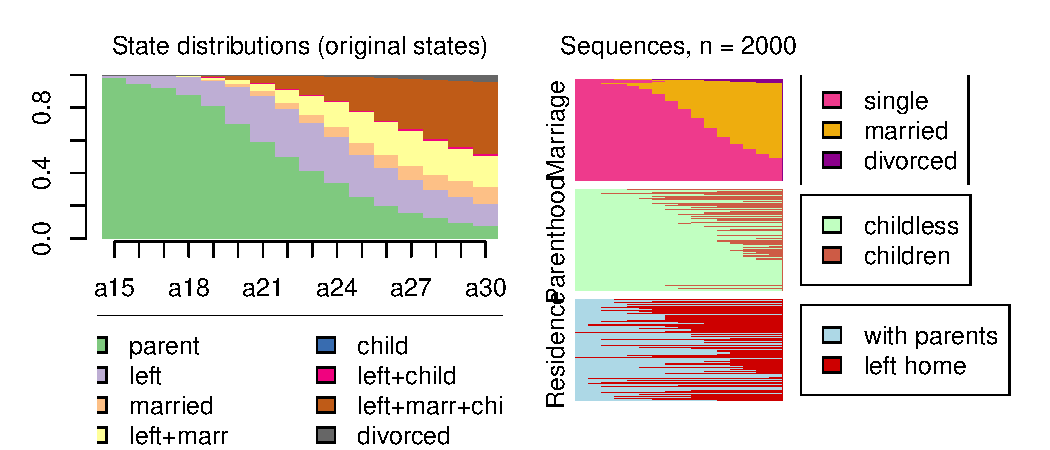
\includegraphics[width=\maxwidth]{figure/gridplot2-1} 

}

\caption[Two different sequence data sets drawn with the \texttt{gridplot} function]{Two different sequence data sets drawn with the \texttt{gridplot} function.}\label{fig:gridplot2}
\end{figure}


\end{knitrout}

\subsection{Converting multichannel to single-channel data}

The \texttt{mc\_to\_sc\_data}\index{MCtoSCdata@\texttt{mc\_to\_sc\_data}} function converts multichannel sequence data to single channel data. At each time point of each individual, the states in each channel are combined into one. Note that here the number of combined observations (10 states) is larger than in the original data (8 states), because we have split the original divorced state into three.

Also single-channel data can be plotted with the \texttt{ssplot}\index{ssplot@\texttt{ssplot}} and  \texttt{gridplot}\index{gridplot@\texttt{gridplot}} functions. Figure \ref{fig:MCtSCdata} illustrates the state distributions. We give more space for the legend to fit the labels, and set new labels for the x axis.

\begin{knitrout}
\definecolor{shadecolor}{rgb}{0.969, 0.969, 0.969}\color{fgcolor}\begin{kframe}
\begin{alltt}
\hlstd{sc_data} \hlkwb{<-} \hlkwd{mc_to_sc_data}\hlstd{(}\hlkwd{list}\hlstd{(marr_seq, child_seq, left_seq))}

\hlkwd{ssplot}\hlstd{(}
  \hlstd{sc_data,} \hlkwc{type} \hlstd{=} \hlstr{"d"}\hlstd{,} \hlkwc{ylab} \hlstd{=} \hlstr{"Proportion"}\hlstd{,} \hlkwc{yaxis} \hlstd{=} \hlnum{TRUE}\hlstd{,}
  \hlkwc{xtlab} \hlstd{=} \hlnum{15}\hlopt{:}\hlnum{30}\hlstd{,} \hlkwc{xlab} \hlstd{=} \hlstr{"Age"}\hlstd{,} \hlkwc{title} \hlstd{=} \hlstr{"Combined states"}\hlstd{,}
  \hlkwc{legend.prop} \hlstd{=} \hlnum{0.4}\hlstd{)}
\end{alltt}
\end{kframe}\begin{figure}

{\centering 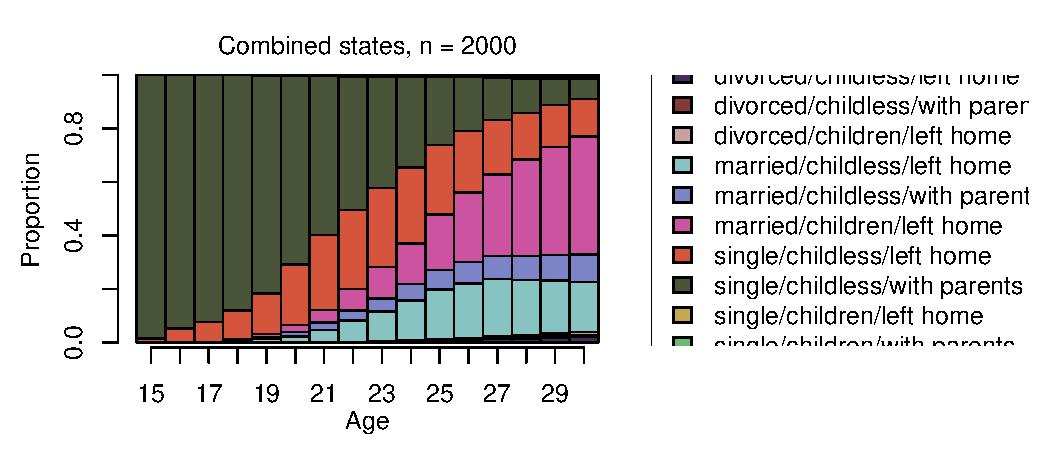
\includegraphics[width=\maxwidth]{figure/MCtSCdata-1} 

}

\caption[Three-channel \texttt{biofam3c} data converted to single-channel data]{Three-channel \texttt{biofam3c} data converted to single-channel data.}\label{fig:MCtSCdata}
\end{figure}


\end{knitrout}



\section{Hidden Markov models}

Hidden Markov models consists of \emph{observed states}, which are regarded as probabilistic functions of \emph{hidden states}. These hidden states cannot be observed directly, but only through the sequence(s) of observations, since they emit the observations on varying probabilities. A discrete first order hidden Markov model for a single sequence can be characterized by the following:

\begin{itemize}
\item \emph{Observed state sequence} $\textbf{y}=(y_1, y_2, \ldots, y_T)$
  with observed states $m\in\{1, \ldots, M\}$.

\item \emph{Hidden state sequence} $\textbf{z}=(z_1, z_2,\ldots, z_T)$
with hidden states $s\in\{1, \ldots, S\}$.

\item \emph{Transition matrix} $A = \{a_{sr}\}$ of size $S \times S$, where $a_{sr}$ is the probability of moving from the hidden state $s$ at time $t-1$ to the hidden state $r$ at time $t$:
        \[a_{sr}	= P(z_t=r|z_{t-1}=s);\quad s,r \in\{1, \ldots, S\}.
				\]
        We only consider homogeneous HMMs where the transition probabilities $a_{sr}$ are constant over time.

\item \emph{Emission matrix} $B=\{b_s(m)\}$ of size $S \times M$ where $b_s(m)$ is the probability of the hidden state $s$ emitting the observed state $m$:
  			\[b_{s}(m)=P(y_t=m|z_t=s); \quad s\in\{1, \ldots, S\}, m\in\{1, \ldots, M\}.
				\]

\item \emph{Initial probability vector} $\pi=\{\pi_s\}$ of length $S$, where $\pi_s$ is the probability of starting from the hidden state $s$:
  			\[\pi_s = P(z_1=s);\quad s\in \{1, \ldots, S\}.
				\]

  \end{itemize}
The (first order) Markov assumption states that the hidden state transition probability at time $t$ only depends on the hidden state at the previous time point $t-1$:
\begin{equation}
P(z_t|z_{t-1},\ldots,z_1)=P(z_t|z_{t-1}).
\end{equation}
Also, the observation at time $t$ is only dependent on the current hidden state, not on previous hidden states or observations:
\begin{equation}
P(y_t|y_{t-1},\ldots,y_1,z_t,\ldots,z_1)=P(y_t|z_t).
\end{equation}

Generalization to case with multiple sequences and multiple channels is straightforward. Sequences $\textbf{y}_i, i=1,\ldots,N$ are assumed to be identically distributed but mutually independent given the states, each individual having their own hidden state sequence. In multichannel case, for each individual $i$ there are $C$ parallel sequences. The model has one transition matrix $A$ but separate emission matrices $B_1,\ldots,B_C$ for each channel. We assume that the observed states in different channels at a given time point $t$ are independent of each other given the hidden state at $t$, i.e. $P(\textbf{y}_{it}|z_{it})=P(y_{it1}|z_{it})\cdots P(y_{itC}|z_{it})$.


Before a HMM can be fitted, the user must define model specifications: the number of hidden states and initial values for parameters for emission, transition, and initial probabilities. Zero values in starting parameters are treated as fixed during the estimation.

We start by showing how HMMs are fitted for the simple single-channel data and then move on to a more complex example with three channels.

\subsection{HMMs for single-channel data}

Our goal here is to fit a model where hidden states describe a more general life stage, during which individuals are more likely to be in certain observable states. We expect that the life stages are somehow related to age, so constructing starting values from observed state frequences by age group seems like an option worth a try. We fit a model with four hidden state using age groups 15--18, 19--23, 24--27, and 28--30. Amount of 0.1 is added to each value in case of zero-frequencies in some categories (at this point we do not want to fix any parameters to zero) and each row is divided with its sum so that the row sums equal to 1.

\begin{knitrout}
\definecolor{shadecolor}{rgb}{0.969, 0.969, 0.969}\color{fgcolor}\begin{kframe}
\begin{alltt}
\hlcom{# Starting values for the emission matrix}
\hlstd{sc_emiss} \hlkwb{<-} \hlkwd{matrix}\hlstd{(}\hlnum{NA}\hlstd{,} \hlkwc{nrow} \hlstd{=} \hlnum{4}\hlstd{,} \hlkwc{ncol} \hlstd{=} \hlnum{8}\hlstd{)}
\hlstd{sc_emiss[}\hlnum{1}\hlstd{,]} \hlkwb{<-} \hlkwd{seqstatf}\hlstd{(biofam.seq[,} \hlnum{1}\hlopt{:}\hlnum{4}\hlstd{])[,} \hlnum{2}\hlstd{]} \hlopt{+} \hlnum{0.1}
\hlstd{sc_emiss[}\hlnum{2}\hlstd{,]} \hlkwb{<-} \hlkwd{seqstatf}\hlstd{(biofam.seq[,} \hlnum{5}\hlopt{:}\hlnum{9}\hlstd{])[,} \hlnum{2}\hlstd{]} \hlopt{+} \hlnum{0.1}
\hlstd{sc_emiss[}\hlnum{3}\hlstd{,]} \hlkwb{<-} \hlkwd{seqstatf}\hlstd{(biofam.seq[,} \hlnum{10}\hlopt{:}\hlnum{13}\hlstd{])[,} \hlnum{2}\hlstd{]} \hlopt{+} \hlnum{0.1}
\hlstd{sc_emiss[}\hlnum{4}\hlstd{,]} \hlkwb{<-} \hlkwd{seqstatf}\hlstd{(biofam.seq[,} \hlnum{14}\hlopt{:}\hlnum{16}\hlstd{])[,} \hlnum{2}\hlstd{]} \hlopt{+} \hlnum{0.1}
\hlstd{sc_emiss} \hlkwb{<-} \hlstd{sc_emiss} \hlopt{/} \hlkwd{rowSums}\hlstd{(sc_emiss)}

\hlcom{# Starting values for the transition matrix}
\hlstd{sc_trans} \hlkwb{<-} \hlkwd{matrix}\hlstd{(}
  \hlkwd{c}\hlstd{(}\hlnum{0.80}\hlstd{,} \hlnum{0.10}\hlstd{,} \hlnum{0.05}\hlstd{,} \hlnum{0.05}\hlstd{,}
    \hlnum{0.05}\hlstd{,} \hlnum{0.80}\hlstd{,} \hlnum{0.10}\hlstd{,} \hlnum{0.05}\hlstd{,}
    \hlnum{0.05}\hlstd{,} \hlnum{0.05}\hlstd{,} \hlnum{0.80}\hlstd{,} \hlnum{0.10}\hlstd{,}
    \hlnum{0.05}\hlstd{,} \hlnum{0.05}\hlstd{,} \hlnum{0.10}\hlstd{,} \hlnum{0.80}\hlstd{),}
  \hlkwc{nrow} \hlstd{=} \hlnum{4}\hlstd{,} \hlkwc{ncol} \hlstd{=} \hlnum{4}\hlstd{,} \hlkwc{byrow} \hlstd{=} \hlnum{TRUE}\hlstd{)}

\hlcom{# Starting values for initial state probabilities}
\hlstd{sc_inits} \hlkwb{<-} \hlkwd{c}\hlstd{(}\hlnum{0.9}\hlstd{,} \hlnum{0.07}\hlstd{,} \hlnum{0.02}\hlstd{,} \hlnum{0.01}\hlstd{)}
\end{alltt}
\end{kframe}
\end{knitrout}
The model is initialized with the \texttt{build\_hmm}\index{buildHMM@\texttt{build\_hmm}} function. It checks that the data and matrices are of the right form and creates an object of class \texttt{hmm}.

\begin{knitrout}
\definecolor{shadecolor}{rgb}{0.969, 0.969, 0.969}\color{fgcolor}\begin{kframe}
\begin{alltt}
\hlcom{# Building a hidden Markov model with starting values}
\hlstd{sc_model} \hlkwb{<-} \hlkwd{build_hmm}\hlstd{(}
  \hlkwc{observations} \hlstd{= biofam.seq,} \hlkwc{transition_probs} \hlstd{= sc_trans,}
  \hlkwc{emission_probs} \hlstd{= sc_emiss,} \hlkwc{initial_probs} \hlstd{= sc_inits)}
\end{alltt}
\end{kframe}
\end{knitrout}
The \texttt{hmm} object can then be fitted with the \texttt{fit\_model}\index{fitHMM@\texttt{fit\_model}} function. The fitting function provides three estimation steps: 1) EM algorithm, 2) global optimization, and 3) local optimization. Any combination of these steps can be chosen but their order cannot be modified. The results from a former step are used as starting values in a latter.

\begin{knitrout}
\definecolor{shadecolor}{rgb}{0.969, 0.969, 0.969}\color{fgcolor}\begin{kframe}
\begin{alltt}
\hlstd{sc_fit} \hlkwb{<-} \hlkwd{fit_model}\hlstd{(sc_model)}
\end{alltt}
\end{kframe}
\end{knitrout}

By default, the \texttt{fit\_model}function starts with a maximum of 1000 iterations of the EM step, skips the global and local L-BFGS optimization steps. For direct numerical estimation (steps 2 and 3), any optimization method available in the \texttt{nloptr} package \citep{nloptr, nlopt} can be chosen.

If the global step is chosen, by default it uses the multilevel single-linkage method (MLSL) \citep{Kan1987I, Kan1987II}. It draws multiple random starting values and performs local optimization from each starting point. The LDS modification uses low-discrepancy sequences instead of random numbers as starting points and should improve the convergence rate \citep{Kucherenko2005}.

There are some theoretical guarantees that the MLSL method shoud find all local optima in a finite number of local optimizations. Of course, it might not always succeed in a reasonable time. Also, it requires setting boundaries for the parameter space, which is not always straightforward. In \texttt{seqHMM} the transition, emission, and initial probabilities are estimated using unconstrained reparameterization using softmax function (a generalization of the logistic function), but good boundaries are essential for efficient use of the MLSL algorithm. If the boundaries are too strict, the global optimum cannot be found; if too wide, the probability of finding the global optimum is decreased. The \texttt{fit\_model}\index{fitHMM@\texttt{fit\_model}} function uses starting values or results from the preciding estimation step to adjust the boundaries. The EM algorithm can help in setting good boundaries, but in some cases it can also lead to worse results. For finding the best solution, it is advisable to try a couple of different settings; e.g. only EM, EM followed by MLSL, a couple of EM iterations followed by MLSL, and only MLSL.

It is also possible to automatically run the EM algorithm multiple times by randomizing starting values. By default, both transition and emission probabilities are modified by adding a random value from the $N(0, 0.25)$ distribution. Although not done by default, this method seems to perform very well as the EM algorithm is relatively fast compared to direct numerical estimation.

For parameter estimation, well known forward--backward recursions are used. As the straightforward implementation of these algorithms pose a great risk of under- and overflow, typically forward probabilities are scaled such that there should be no underflow. Although this is often sufficient for forward algorithm, this can result an overflow problem in backward algorithm where the same scaling factors are used. Thus in addition to scaling approach, \texttt{seqHMM} supports logarithm scale for most of the computations, which further reduces the numerical unstabilities. On the other hand, as there is a need to back-transform to natural scale during the algorithms, the log-space approach seems to be typically about 3--4 times slower than scaling approach. Therefore by default all functions use the scaling approach, whereas the log-space approach can be used by setting argument \texttt{log\_space} to \texttt{TRUE}.

Most of the functions relating to model estimation and state inference support parallel computation via OpenMP interface. The user can choose the number of parallel threads (e.g. the number of cores) to use for the specific task. By default, no parallelization is done.


The \texttt{fit\_model}\index{fitHMM@\texttt{fit\_model}} function returns the model, the log-likelihood, and estimation results from each step.

\begin{knitrout}
\definecolor{shadecolor}{rgb}{0.969, 0.969, 0.969}\color{fgcolor}\begin{kframe}
\begin{alltt}
\hlstd{sc_fit}\hlopt{$}\hlstd{model}
\end{alltt}
\begin{verbatim}
## Initial probabilities :
## State 1 State 2 State 3 State 4 
##   0.986   0.014   0.000   0.000 
## 
## Transition probabilities :
##          to
## from      State 1 State 2 State 3 State 4
##   State 1   0.886  0.0546 0.03220  0.0275
##   State 2   0.000  0.8898 0.08342  0.0267
##   State 3   0.000  0.0000 0.78724  0.2128
##   State 4   0.000  0.0000 0.00136  0.9986
## 
## Emission probabilities :
##            symbol_names
## state_names 0 1       2     3       4      5     6      7
##     State 1 1 0 0.00000 0.000 0.00000 0.0000 0.000 0.0000
##     State 2 0 1 0.00000 0.000 0.00000 0.0000 0.000 0.0000
##     State 3 0 0 0.00194 0.998 0.00000 0.0000 0.000 0.0000
##     State 4 0 0 0.21448 0.000 0.00279 0.0245 0.711 0.0473
\end{verbatim}
\end{kframe}
\end{knitrout}

\subsection{HMMs for multichannel data}

A HMM for multichannel data is fitted in a similar way using the same \texttt{build\_hmm}\index{buildHMM@\texttt{build\_hmm}} and \texttt{fit\_model}\index{fitHMM@\texttt{fit\_model}} functions. Now we build a model for three-channel data with four hidden states. One emission matrix (with hidden states as rows and observed states as columns) is required for each channel, i.e. 4x3 matrix for marriages and 4x2 matrices for the other two. Also here the initial values are constructed from using the observed state frequences at different age categories (see the example of fitting HMM for single-channel data). Now we use an upper triangular matrix in the transition matrix indicating a left-to-right model where transitions back to previous states are not allowed. This seems like a valid option from a life-course prespective. Also, in the previous single-channel model of the same data the transition matrix was estimated almost upper triangular.

\begin{knitrout}
\definecolor{shadecolor}{rgb}{0.969, 0.969, 0.969}\color{fgcolor}\begin{kframe}
\begin{alltt}
\hlcom{# Initial values for initial state probabilities}
\hlstd{mc_inits} \hlkwb{<-} \hlkwd{c}\hlstd{(}\hlnum{0.90}\hlstd{,} \hlnum{0.07}\hlstd{,} \hlnum{0.02}\hlstd{,} \hlnum{0.01}\hlstd{)}

\hlcom{# Initial values for transition matrix}
\hlstd{mc_trans} \hlkwb{<-} \hlkwd{matrix}\hlstd{(}
  \hlkwd{c}\hlstd{(}\hlnum{0.90}\hlstd{,} \hlnum{0.06}\hlstd{,} \hlnum{0.03}\hlstd{,} \hlnum{0.01}\hlstd{,}
       \hlnum{0}\hlstd{,} \hlnum{0.90}\hlstd{,} \hlnum{0.07}\hlstd{,} \hlnum{0.03}\hlstd{,}
       \hlnum{0}\hlstd{,}    \hlnum{0}\hlstd{,} \hlnum{0.90}\hlstd{,} \hlnum{0.10}\hlstd{,}
       \hlnum{0}\hlstd{,}    \hlnum{0}\hlstd{,}    \hlnum{0}\hlstd{,}    \hlnum{1}\hlstd{),}
  \hlkwc{nrow} \hlstd{=} \hlnum{4}\hlstd{,} \hlkwc{ncol} \hlstd{=} \hlnum{4}\hlstd{,} \hlkwc{byrow} \hlstd{=} \hlnum{TRUE}\hlstd{)}

\hlcom{# Initial values for emission matrices}
\hlstd{mc_B_marr} \hlkwb{<-} \hlkwd{matrix}\hlstd{(}\hlnum{NA}\hlstd{,} \hlkwc{nrow} \hlstd{=} \hlnum{4}\hlstd{,} \hlkwc{ncol} \hlstd{=} \hlnum{3}\hlstd{)}
\hlstd{mc_B_marr[}\hlnum{1}\hlstd{,]} \hlkwb{<-} \hlkwd{seqstatf}\hlstd{(marr_seq[,} \hlnum{1}\hlopt{:}\hlnum{4}\hlstd{])[,} \hlnum{2}\hlstd{]} \hlopt{+} \hlnum{1}
\hlstd{mc_B_marr[}\hlnum{2}\hlstd{,]} \hlkwb{<-} \hlkwd{seqstatf}\hlstd{(marr_seq[,} \hlnum{5}\hlopt{:}\hlnum{8}\hlstd{])[,} \hlnum{2}\hlstd{]} \hlopt{+} \hlnum{1}
\hlstd{mc_B_marr[}\hlnum{3}\hlstd{,]} \hlkwb{<-} \hlkwd{seqstatf}\hlstd{(marr_seq[,} \hlnum{9}\hlopt{:}\hlnum{12}\hlstd{])[,} \hlnum{2}\hlstd{]} \hlopt{+} \hlnum{1}
\hlstd{mc_B_marr[}\hlnum{4}\hlstd{,]} \hlkwb{<-} \hlkwd{seqstatf}\hlstd{(marr_seq[,} \hlnum{13}\hlopt{:}\hlnum{16}\hlstd{])[,} \hlnum{2}\hlstd{]} \hlopt{+} \hlnum{1}
\hlstd{mc_B_marr} \hlkwb{<-} \hlstd{mc_B_marr} \hlopt{/} \hlkwd{rowSums}\hlstd{(mc_B_marr)}

\hlstd{mc_B_child} \hlkwb{<-} \hlkwd{matrix}\hlstd{(}\hlnum{NA}\hlstd{,} \hlkwc{nrow} \hlstd{=} \hlnum{4}\hlstd{,} \hlkwc{ncol} \hlstd{=} \hlnum{2}\hlstd{)}
\hlstd{mc_B_child[}\hlnum{1}\hlstd{,]} \hlkwb{<-} \hlkwd{seqstatf}\hlstd{(child_seq[,} \hlnum{1}\hlopt{:}\hlnum{4}\hlstd{])[,} \hlnum{2}\hlstd{]} \hlopt{+} \hlnum{1}
\hlstd{mc_B_child[}\hlnum{2}\hlstd{,]} \hlkwb{<-} \hlkwd{seqstatf}\hlstd{(child_seq[,} \hlnum{5}\hlopt{:}\hlnum{8}\hlstd{])[,} \hlnum{2}\hlstd{]} \hlopt{+} \hlnum{1}
\hlstd{mc_B_child[}\hlnum{3}\hlstd{,]} \hlkwb{<-} \hlkwd{seqstatf}\hlstd{(child_seq[,} \hlnum{9}\hlopt{:}\hlnum{12}\hlstd{])[,} \hlnum{2}\hlstd{]} \hlopt{+} \hlnum{1}
\hlstd{mc_B_child[}\hlnum{4}\hlstd{,]} \hlkwb{<-} \hlkwd{seqstatf}\hlstd{(child_seq[,} \hlnum{13}\hlopt{:}\hlnum{16}\hlstd{])[,} \hlnum{2}\hlstd{]} \hlopt{+} \hlnum{1}
\hlstd{mc_B_child} \hlkwb{<-} \hlstd{mc_B_child} \hlopt{/} \hlkwd{rowSums}\hlstd{(mc_B_child)}

\hlstd{mc_B_left} \hlkwb{<-} \hlkwd{matrix}\hlstd{(}\hlnum{NA}\hlstd{,} \hlkwc{nrow} \hlstd{=} \hlnum{4}\hlstd{,} \hlkwc{ncol} \hlstd{=} \hlnum{2}\hlstd{)}
\hlstd{mc_B_left[}\hlnum{1}\hlstd{,]} \hlkwb{<-} \hlkwd{seqstatf}\hlstd{(left_seq[,} \hlnum{1}\hlopt{:}\hlnum{4}\hlstd{])[,} \hlnum{2}\hlstd{]} \hlopt{+} \hlnum{0.1}
\hlstd{mc_B_left[}\hlnum{2}\hlstd{,]} \hlkwb{<-} \hlkwd{seqstatf}\hlstd{(left_seq[,} \hlnum{5}\hlopt{:}\hlnum{8}\hlstd{])[,} \hlnum{2}\hlstd{]} \hlopt{+} \hlnum{0.1}
\hlstd{mc_B_left[}\hlnum{3}\hlstd{,]} \hlkwb{<-} \hlkwd{seqstatf}\hlstd{(left_seq[,} \hlnum{9}\hlopt{:}\hlnum{12}\hlstd{])[,} \hlnum{2}\hlstd{]} \hlopt{+} \hlnum{0.1}
\hlstd{mc_B_left[}\hlnum{4}\hlstd{,]} \hlkwb{<-} \hlkwd{seqstatf}\hlstd{(left_seq[,} \hlnum{13}\hlopt{:}\hlnum{16}\hlstd{])[,} \hlnum{2}\hlstd{]} \hlopt{+} \hlnum{0.1}
\hlstd{mc_B_left} \hlkwb{<-} \hlstd{mc_B_left} \hlopt{/} \hlkwd{rowSums}\hlstd{(mc_B_left)}

\hlcom{# Build HMM}
\hlstd{mc_hmm} \hlkwb{<-} \hlkwd{build_hmm}\hlstd{(}
  \hlkwc{observations} \hlstd{=} \hlkwd{list}\hlstd{(marr_seq, child_seq, left_seq),}
  \hlkwc{initial_probs} \hlstd{= mc_inits,} \hlkwc{transition_probs} \hlstd{= mc_trans,}
  \hlkwc{emission_probs} \hlstd{=} \hlkwd{list}\hlstd{(mc_B_marr, mc_B_child, mc_B_left),}
  \hlkwc{channel_names} \hlstd{=} \hlkwd{c}\hlstd{(}\hlstr{"Marriage"}\hlstd{,} \hlstr{"Parenthood"}\hlstd{,} \hlstr{"Residence"}\hlstd{))}

\hlcom{# Fit HMM}
\hlstd{mc_fit} \hlkwb{<-} \hlkwd{fit_model}\hlstd{(mc_hmm,} \hlkwc{local} \hlstd{=} \hlnum{TRUE}\hlstd{)}
\end{alltt}
\end{kframe}
\end{knitrout}

\subsection{Evaluating and comparing HMMs}

\subsubsection{Log-likelihood}

Log-likelihood is stored in the result from \texttt{fit\_model}\index{fitHMM@\texttt{fit\_model}}, but also the \texttt{logLik}\index{logLik@\texttt{logLik}} function computes it. Models with the same number of parameters can be compared using log-likelihood: the bigger the value, the better the model.

\begin{knitrout}
\definecolor{shadecolor}{rgb}{0.969, 0.969, 0.969}\color{fgcolor}\begin{kframe}
\begin{alltt}
\hlstd{mc_fit}\hlopt{$}\hlstd{logLik}
\end{alltt}
\begin{verbatim}
## [1] -16854.16
\end{verbatim}
\begin{alltt}
\hlkwd{logLik}\hlstd{(mc_fit}\hlopt{$}\hlstd{model)}
\end{alltt}
\begin{verbatim}
## 'log Lik.' -16854.16 (df=25)
\end{verbatim}
\end{kframe}
\end{knitrout}

Next we fit a couple of models with different estimation procedures and compare the results using log-likelihood. We first note that for this model the EM algorithm converges to optimum so the local optimization step is not necessary (the difference between the log-likelihoods is neglibigle, -2.8e-9):

\begin{knitrout}
\definecolor{shadecolor}{rgb}{0.969, 0.969, 0.969}\color{fgcolor}\begin{kframe}
\begin{alltt}
\hlstd{mc_fit}\hlopt{$}\hlstd{em_results}\hlopt{$}\hlstd{logLik}
\end{alltt}
\begin{verbatim}
## [1] -16854.16
\end{verbatim}
\begin{alltt}
\hlopt{-}\hlstd{mc_fit}\hlopt{$}\hlstd{local_results}\hlopt{$}\hlstd{objective}
\end{alltt}
\begin{verbatim}
## [1] -16854.16
\end{verbatim}
\end{kframe}
\end{knitrout}

Using only gradient-based optimization without the initial EM step produces slightly poorer fit:
\begin{knitrout}
\definecolor{shadecolor}{rgb}{0.969, 0.969, 0.969}\color{fgcolor}\begin{kframe}
\begin{alltt}
\hlstd{mc_fit_local} \hlkwb{<-} \hlkwd{fit_model}\hlstd{(mc_hmm,} \hlkwc{em_step} \hlstd{=} \hlnum{FALSE}\hlstd{,} \hlkwc{local} \hlstd{=} \hlnum{TRUE}\hlstd{)}
\hlstd{mc_fit_local}\hlopt{$}\hlstd{logLik}
\end{alltt}
\begin{verbatim}
## [1] -16854.34
\end{verbatim}
\end{kframe}
\end{knitrout}

Next we will test the performance of the MLSL optimization by setting \texttt{global = TRUE}. Final polishing is done with the L-BFGS. The default estimation time is set to 60 seconds in global step, but usually it is advisable to run it longer. Depending on the performance of the computer, the optimizer may also be able to perform more or less evaluations in the given time limit. Setting \texttt{maxtime = 0} omits the time limit and performs the number of evaluations given for \texttt{maxeval}. The more complex the model, the more time the optimizer needs to throughly search the parameter space. Here we use parallel computing with 4 threads in order to speed up the computations.

\begin{knitrout}
\definecolor{shadecolor}{rgb}{0.969, 0.969, 0.969}\color{fgcolor}\begin{kframe}
\begin{alltt}
\hlstd{mc_fit_global} \hlkwb{<-} \hlkwd{fit_model}\hlstd{(mc_hmm,} \hlkwc{em_step} \hlstd{=} \hlnum{FALSE}\hlstd{,}
  \hlkwc{global} \hlstd{=} \hlnum{TRUE}\hlstd{,} \hlkwc{local} \hlstd{=} \hlnum{TRUE}\hlstd{,} \hlkwc{threads} \hlstd{=} \hlnum{4}\hlstd{,}
  \hlkwc{control_global} \hlstd{=} \hlkwd{list}\hlstd{(}\hlkwc{maxtime} \hlstd{=} \hlnum{0}\hlstd{,} \hlkwc{maxeval} \hlstd{=} \hlnum{10000}\hlstd{))}

\hlopt{-}\hlstd{mc_fit_global}\hlopt{$}\hlstd{global_results}\hlopt{$}\hlstd{objective}
\end{alltt}
\begin{verbatim}
## [1] -16854.35
\end{verbatim}
\begin{alltt}
\hlopt{-}\hlstd{mc_fit_global}\hlopt{$}\hlstd{local_results}\hlopt{$}\hlstd{objective}
\end{alltt}
\begin{verbatim}
## [1] -16854.35
\end{verbatim}
\end{kframe}
\end{knitrout}

In this case, even when using 10000 iterations the global optimization still does not find the same optimum as the EM algorithm. Note that in order to minimize the time spend on suboptimal regions of parameter space, by default the global optimization step uses larger relative tolerances in internal local optimization phases than the subsequent local optimization step. Also MLSL does not use the initial values at start of the optimization (except in setting the boundaries of parameter space), so it can miss the optimum found by local optimization only.

Automatic restarts of the EM algorithm are called by setting the argument \texttt{restart} in the \texttt{control\_em} argument. By default, both transition and emission probabilities are modified by adding a random numbers from a normal distribution with a mean of 0 and a standard error defined by \texttt{sd} (0.25 by default). Rows of matrices are then scaled to sum to one. Here randomizing is only useful for a check-up since the original EM already seems find the global optimum.

\begin{knitrout}
\definecolor{shadecolor}{rgb}{0.969, 0.969, 0.969}\color{fgcolor}\begin{kframe}
\begin{alltt}
\hlkwd{set.seed}\hlstd{(}\hlnum{123}\hlstd{)}
\hlstd{mc_hmm_restarts} \hlkwb{<-} \hlkwd{fit_model}\hlstd{(mc_hmm,}
  \hlkwc{control_em} \hlstd{=} \hlkwd{list}\hlstd{(}\hlkwc{restart} \hlstd{=} \hlkwd{list}\hlstd{(}\hlkwc{times} \hlstd{=} \hlnum{100}\hlstd{,} \hlkwc{transition} \hlstd{=} \hlnum{FALSE}\hlstd{)))}
\hlstd{mc_hmm_restarts}\hlopt{$}\hlstd{logLik}
\end{alltt}
\begin{verbatim}
## [1] -16854.16
\end{verbatim}
\end{kframe}
\end{knitrout}

\subsubsection{Bayesian information criterion (BIC)}

The \texttt{BIC}\index{BIC@\texttt{BIC}} function gives the value of the Bayesian information criterion (BIC).

\begin{knitrout}
\definecolor{shadecolor}{rgb}{0.969, 0.969, 0.969}\color{fgcolor}\begin{kframe}
\begin{alltt}
\hlkwd{BIC}\hlstd{(mc_fit}\hlopt{$}\hlstd{model)}
\end{alltt}
\begin{verbatim}
## [1] 33967.66
\end{verbatim}
\end{kframe}
\end{knitrout}
BIC can be used to compare models with a different number of parameters, e.g. for choosing the best number of hidden states. We fit a model with three hidden states and compare the results to the four-state model.

\begin{knitrout}
\definecolor{shadecolor}{rgb}{0.969, 0.969, 0.969}\color{fgcolor}\begin{kframe}
\begin{alltt}
\hlstd{mc_inits_3s} \hlkwb{<-} \hlkwd{c}\hlstd{(}\hlnum{0.90}\hlstd{,} \hlnum{0.07}\hlstd{,} \hlnum{0.03}\hlstd{)}

\hlstd{mc_A_3s} \hlkwb{<-} \hlkwd{matrix}\hlstd{(}
  \hlkwd{c}\hlstd{(}\hlnum{0.90}\hlstd{,} \hlnum{0.07}\hlstd{,} \hlnum{0.03}\hlstd{,}
       \hlnum{0}\hlstd{,} \hlnum{0.90}\hlstd{,} \hlnum{0.10}\hlstd{,}
       \hlnum{0}\hlstd{,}    \hlnum{0}\hlstd{,}    \hlnum{1}\hlstd{),}
  \hlkwc{nrow} \hlstd{=} \hlnum{3}\hlstd{,} \hlkwc{ncol} \hlstd{=} \hlnum{3}\hlstd{,} \hlkwc{byrow} \hlstd{=} \hlnum{TRUE}\hlstd{)}

\hlstd{mc_B_marr_3s} \hlkwb{<-} \hlkwd{matrix}\hlstd{(}\hlnum{NA}\hlstd{,} \hlkwc{nrow}\hlstd{=}  \hlnum{3}\hlstd{,} \hlkwc{ncol} \hlstd{=} \hlnum{3}\hlstd{)}
\hlstd{mc_B_marr_3s[}\hlnum{1}\hlstd{,]} \hlkwb{<-} \hlkwd{seqstatf}\hlstd{(marr_seq[,} \hlnum{1}\hlopt{:}\hlnum{5}\hlstd{])[,} \hlnum{2}\hlstd{]} \hlopt{+} \hlnum{0.1}
\hlstd{mc_B_marr_3s[}\hlnum{2}\hlstd{,]} \hlkwb{<-} \hlkwd{seqstatf}\hlstd{(marr_seq[,} \hlnum{6}\hlopt{:}\hlnum{10}\hlstd{])[,} \hlnum{2}\hlstd{]} \hlopt{+} \hlnum{0.1}
\hlstd{mc_B_marr_3s[}\hlnum{3}\hlstd{,]} \hlkwb{<-} \hlkwd{seqstatf}\hlstd{(marr_seq[,} \hlnum{11}\hlopt{:}\hlnum{16}\hlstd{])[,} \hlnum{2}\hlstd{]} \hlopt{+} \hlnum{0.1}
\hlstd{mc_B_marr_3s} \hlkwb{<-} \hlstd{mc_B_marr_3s} \hlopt{/} \hlkwd{rowSums}\hlstd{(mc_B_marr_3s)}

\hlstd{mc_B_child_3s} \hlkwb{<-} \hlkwd{matrix}\hlstd{(}\hlnum{NA}\hlstd{,} \hlkwc{nrow} \hlstd{=} \hlnum{3}\hlstd{,} \hlkwc{ncol} \hlstd{=} \hlnum{2}\hlstd{)}
\hlstd{mc_B_child_3s[}\hlnum{1}\hlstd{,]} \hlkwb{<-} \hlkwd{seqstatf}\hlstd{(child_seq[,} \hlnum{1}\hlopt{:}\hlnum{5}\hlstd{])[,} \hlnum{2}\hlstd{]} \hlopt{+} \hlnum{0.1}
\hlstd{mc_B_child_3s[}\hlnum{2}\hlstd{,]} \hlkwb{<-} \hlkwd{seqstatf}\hlstd{(child_seq[,} \hlnum{6}\hlopt{:}\hlnum{10}\hlstd{])[,} \hlnum{2}\hlstd{]} \hlopt{+} \hlnum{0.1}
\hlstd{mc_B_child_3s[}\hlnum{3}\hlstd{,]} \hlkwb{<-} \hlkwd{seqstatf}\hlstd{(child_seq[,} \hlnum{11}\hlopt{:}\hlnum{16}\hlstd{])[,} \hlnum{2}\hlstd{]} \hlopt{+} \hlnum{0.1}
\hlstd{mc_B_child_3s} \hlkwb{<-} \hlstd{mc_B_child_3s} \hlopt{/} \hlkwd{rowSums}\hlstd{(mc_B_child_3s)}

\hlstd{mc_B_left_3s} \hlkwb{<-} \hlkwd{matrix}\hlstd{(}\hlnum{NA}\hlstd{,} \hlkwc{nrow} \hlstd{=} \hlnum{3}\hlstd{,} \hlkwc{ncol} \hlstd{=} \hlnum{2}\hlstd{)}
\hlstd{mc_B_left_3s[}\hlnum{1}\hlstd{,]} \hlkwb{<-} \hlkwd{seqstatf}\hlstd{(left_seq[,} \hlnum{1}\hlopt{:}\hlnum{5}\hlstd{])[,} \hlnum{2}\hlstd{]} \hlopt{+} \hlnum{0.1}
\hlstd{mc_B_left_3s[}\hlnum{2}\hlstd{,]} \hlkwb{<-} \hlkwd{seqstatf}\hlstd{(left_seq[,} \hlnum{6}\hlopt{:}\hlnum{10}\hlstd{])[,} \hlnum{2}\hlstd{]} \hlopt{+} \hlnum{0.1}
\hlstd{mc_B_left_3s[}\hlnum{3}\hlstd{,]} \hlkwb{<-} \hlkwd{seqstatf}\hlstd{(left_seq[,} \hlnum{11}\hlopt{:}\hlnum{16}\hlstd{])[,} \hlnum{2}\hlstd{]} \hlopt{+} \hlnum{0.1}
\hlstd{mc_B_left_3s} \hlkwb{<-} \hlstd{mc_B_left_3s} \hlopt{/} \hlkwd{rowSums}\hlstd{(mc_B_left_3s)}

\hlstd{mc_hmm_3s} \hlkwb{<-} \hlkwd{build_hmm}\hlstd{(}
  \hlkwc{observations} \hlstd{=} \hlkwd{list}\hlstd{(marr_seq, child_seq, left_seq),}
  \hlkwc{initial_probs} \hlstd{= mc_inits_3s,} \hlkwc{transition_probs} \hlstd{= mc_A_3s,}
  \hlkwc{emission_probs} \hlstd{=} \hlkwd{list}\hlstd{(mc_B_marr_3s, mc_B_child_3s, mc_B_left_3s),}
  \hlkwc{channel_names} \hlstd{=} \hlkwd{c}\hlstd{(}\hlstr{"Marriage"}\hlstd{,} \hlstr{"Parenthood"}\hlstd{,} \hlstr{"Residence"}\hlstd{))}

\hlstd{mc_fit_3s} \hlkwb{<-} \hlkwd{fit_model}\hlstd{(mc_hmm_3s)}

\hlstd{mc_fit_3s}\hlopt{$}\hlstd{logLik}
\end{alltt}
\begin{verbatim}
## [1] -22617.08
\end{verbatim}
\begin{alltt}
\hlkwd{BIC}\hlstd{(mc_fit_3s}\hlopt{$}\hlstd{model)}
\end{alltt}
\begin{verbatim}
## [1] 45410.52
\end{verbatim}
\end{kframe}
\end{knitrout}
BIC for the four-state model is 33967.66, which is less than 45410.52, BIC for the three-state model. We can conclude (assuming that we found the global optimum in both cases), that the model with four hidden states is better.

\subsection{Converting multichannel models to single-channel models}

The \texttt{mc\_to\_sc}\index{MCtoSC@\texttt{mc\_to\_sc}} function converts multichannel models to single-channel representations. It combines observed states and multiplies emission parameters across channels. Instead of three emission matrices of size $4\times 3$, $4\times 2$, and $4\times 2$ we now have one emission matrix of size $4\times 10$, since there are 10 state combinations in the new data.

\begin{knitrout}
\definecolor{shadecolor}{rgb}{0.969, 0.969, 0.969}\color{fgcolor}\begin{kframe}
\begin{alltt}
\hlstd{sc_hmm} \hlkwb{<-} \hlkwd{mc_to_sc}\hlstd{(mc_fit}\hlopt{$}\hlstd{model)}
\end{alltt}
\end{kframe}
\end{knitrout}


\section{Plotting hidden Markov models}

When the function is fitted, the \texttt{hmm} object can be easily plotted as a directed graph with the \texttt{plot}\index{plot.hmm@\texttt{plot.hmm}} method. By default, each hidden state is represented as a pie chart with the (combinations of) emitted states as slices. States with emission probability less than 0.05 are combined into one category, unless the user specifies otherwise. By default, the initial state probabilities are given below the vertices, and the widths of the edges giving the transition probabilities vary according to the parameter values. If the \texttt{hmm} object has multiple channels, the \texttt{mc\_to\_sc}\index{MCtoSC@\texttt{mc\_to\_sc}} function is automatically used to convert the multichannel model into a single channel model during plotting. Figure \ref{fig:plotHMM1} illustrates a default plot for the four-state model fitted earlier.

\begin{knitrout}
\definecolor{shadecolor}{rgb}{0.969, 0.969, 0.969}\color{fgcolor}\begin{kframe}
\begin{alltt}
\hlkwd{plot}\hlstd{(mc_fit}\hlopt{$}\hlstd{model)}
\end{alltt}
\end{kframe}\begin{figure}
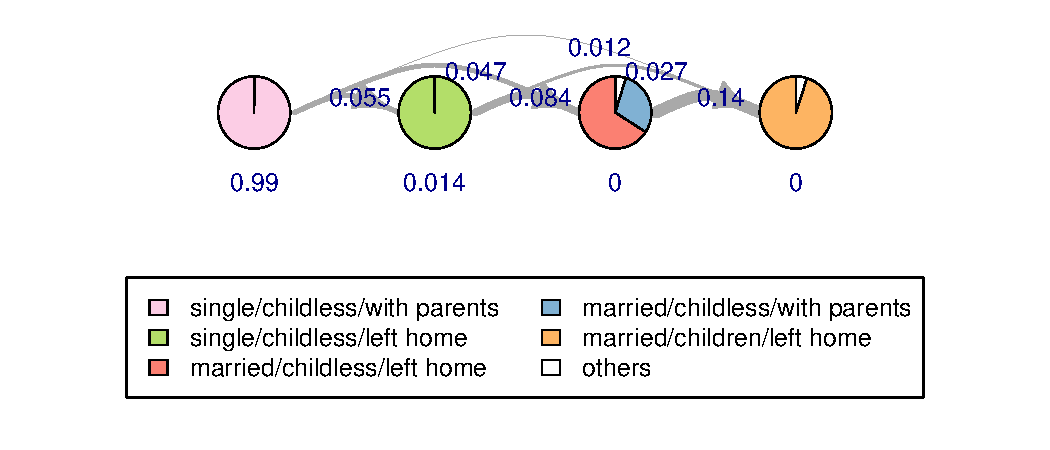
\includegraphics[width=\maxwidth]{figure/plotHMM1-1} \caption[Plotting HMM as a directed graph with the \texttt{plot} method]{Plotting HMM as a directed graph with the \texttt{plot} method.}\label{fig:plotHMM1}
\end{figure}


\end{knitrout}

The \texttt{hmm} plots can be modified in various ways such as changing sizes and positions of vertices, thickness and curvature of edges, colors and fonts of labels, and position and contents of the legend. The \texttt{igraph} package \citep{Csardi2006} is used for plotting directed graphs, so most arguments of the \texttt{plot.igraph} function work in \texttt{plot.hmm} as well. In Figure \ref{fig:plotHMM2} we draw bigger vertices, modify the legend, change curvatures of edges, and give a new label for the combined slice.

\begin{knitrout}
\definecolor{shadecolor}{rgb}{0.969, 0.969, 0.969}\color{fgcolor}\begin{kframe}
\begin{alltt}
\hlkwd{plot}\hlstd{(}
  \hlstd{mc_fit}\hlopt{$}\hlstd{model,} \hlkwc{vertex.size} \hlstd{=} \hlnum{50}\hlstd{,} \hlkwc{ncol.legend} \hlstd{=} \hlnum{2}\hlstd{,} \hlkwc{legend.prop} \hlstd{=} \hlnum{0.4}\hlstd{,}
  \hlkwc{edge.curved} \hlstd{=} \hlkwd{c}\hlstd{(}\hlnum{0}\hlstd{,} \hlnum{0.7}\hlstd{,} \hlopt{-}\hlnum{0.6}\hlstd{,} \hlnum{0}\hlstd{,} \hlnum{0.7}\hlstd{,} \hlnum{0}\hlstd{),}
  \hlkwc{combined.slice.label} \hlstd{=} \hlstr{"States with probability < 0.05"}\hlstd{)}
\end{alltt}
\end{kframe}\begin{figure}
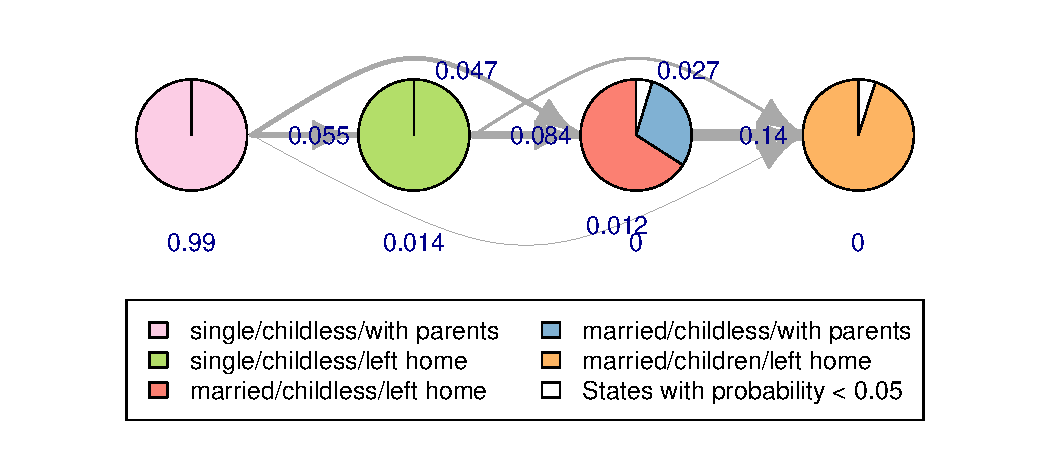
\includegraphics[width=\maxwidth]{figure/plotHMM2-1} \caption{Another version of the same model as in Figure \ref{fig:plotHMM1}.}\label{fig:plotHMM2}
\end{figure}


\end{knitrout}

By default, the vertices are plotted vertically aligned but that can be changed with the \texttt{layout} argument. Ready-made options include horizontal and vertical positioning, but also coordinates and layout functions of the \texttt{igraph} package can be given to position the vertices. Coordinates are given in a two-column matrix, with x coordinates in the first column and y coordinates in the second. Arguments \texttt{xlim} and \texttt{ylim} set the lengths of the axes and \texttt{rescale = FALSE} prevents rescaling the coordinates to the $[-1,1]\times[-1,1]$ interval (the default).

In Figure \ref{fig:plotHMM3} we change the positions of the vertex labels (initial probabilities), call for straight and thinner edges with smaller arrows, modify the legend, ask to plot all emitted states, and change colors.

\begin{knitrout}
\definecolor{shadecolor}{rgb}{0.969, 0.969, 0.969}\color{fgcolor}\begin{kframe}
\begin{alltt}
\hlkwd{plot}\hlstd{(}
  \hlstd{mc_fit}\hlopt{$}\hlstd{model,}
  \hlkwc{layout} \hlstd{=} \hlkwd{matrix}\hlstd{(}\hlkwd{c}\hlstd{(}\hlnum{1}\hlstd{,}\hlnum{3}\hlstd{,}\hlnum{3}\hlstd{,}\hlnum{5}\hlstd{,}
                    \hlnum{0}\hlstd{,}\hlopt{-}\hlnum{1}\hlstd{,}\hlnum{1}\hlstd{,}\hlnum{0}\hlstd{),} \hlkwc{ncol} \hlstd{=} \hlnum{2}\hlstd{),}
  \hlkwc{xlim} \hlstd{=} \hlkwd{c}\hlstd{(}\hlnum{0.5}\hlstd{,} \hlnum{5.5}\hlstd{),} \hlkwc{ylim} \hlstd{=} \hlkwd{c}\hlstd{(}\hlopt{-}\hlnum{1.5}\hlstd{,} \hlnum{1.5}\hlstd{),} \hlkwc{rescale} \hlstd{=} \hlnum{FALSE}\hlstd{,}
  \hlkwc{vertex.size} \hlstd{=} \hlnum{50}\hlstd{,} \hlkwc{vertex.label.pos} \hlstd{=} \hlkwd{c}\hlstd{(pi, pi}\hlopt{/}\hlnum{2}\hlstd{,} \hlopt{-}\hlstd{pi}\hlopt{/}\hlnum{2}\hlstd{,} \hlnum{0}\hlstd{),}
  \hlkwc{edge.curved} \hlstd{=} \hlnum{FALSE}\hlstd{,} \hlkwc{cex.edge.width} \hlstd{=} \hlnum{0.8}\hlstd{,} \hlkwc{edge.arrow.size} \hlstd{=} \hlnum{1.2}\hlstd{,}
  \hlkwc{withlegend} \hlstd{=} \hlstr{"top"}\hlstd{,} \hlkwc{legend.prop} \hlstd{=} \hlnum{0.3}\hlstd{,} \hlkwc{cex.legend} \hlstd{=} \hlnum{1.1}\hlstd{,} \hlkwc{ncol.legend} \hlstd{=} \hlnum{2}\hlstd{,}
  \hlkwc{combine.slices} \hlstd{=} \hlnum{0}\hlstd{,} \hlkwc{cpal} \hlstd{= colorpalette[[}\hlnum{15}\hlstd{]][}\hlnum{1}\hlopt{:}\hlnum{10}\hlstd{])}
\end{alltt}
\end{kframe}\begin{figure}
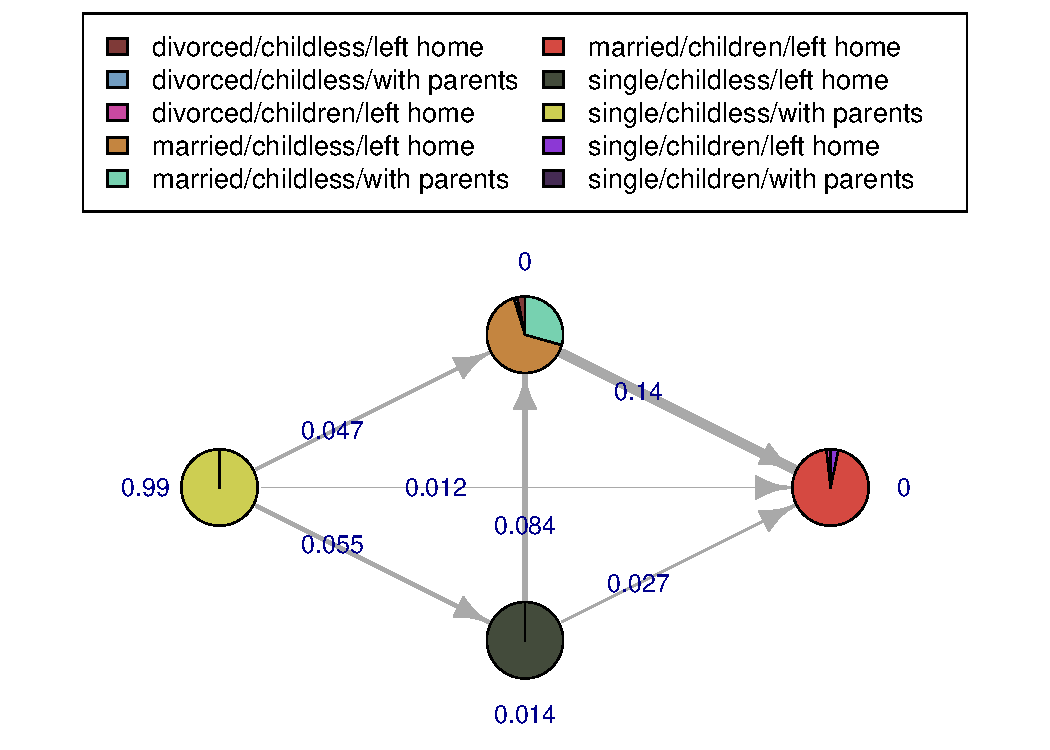
\includegraphics[width=\maxwidth]{figure/plotHMM3-1} \caption{Another version of the same model as in Figure \ref{fig:plotHMM1}.}\label{fig:plotHMM3}
\end{figure}


\end{knitrout}

A color must be provided for all (combinations of) observed states present in the data, whether or not shown in the graph. The \texttt{seqHMM} package uses the \texttt{colorpalette}\index{colorpalette@\texttt{colorpalette}} data for defining the colors in the plots. It is a list of 60 ready-made color palettes with 1--60 distinct colors and is automatically loaded with the package and available for use. See also the \texttt{RColorBrewer} package for more color palettes with distinct colors. The \texttt{plot\_colors}\index{plotcolors@\texttt{plot\_colors}} function is provided fot easy visualization of color palettes.

\begin{knitrout}
\definecolor{shadecolor}{rgb}{0.969, 0.969, 0.969}\color{fgcolor}\begin{kframe}
\begin{alltt}
\hlkwd{plot_colors}\hlstd{(colorpalette[[}\hlnum{8}\hlstd{]],}
  \hlkwc{labels} \hlstd{=} \hlkwd{c}\hlstd{(}\hlstr{"parent"}\hlstd{,} \hlstr{"left"}\hlstd{,} \hlstr{"married"}\hlstd{,} \hlstr{"left+marr"}\hlstd{,} \hlstr{"child"}\hlstd{,}
             \hlstr{"left+child"}\hlstd{,} \hlstr{"left+marr+child"}\hlstd{,} \hlstr{"divorced"}\hlstd{))}
\end{alltt}
\end{kframe}\begin{figure}
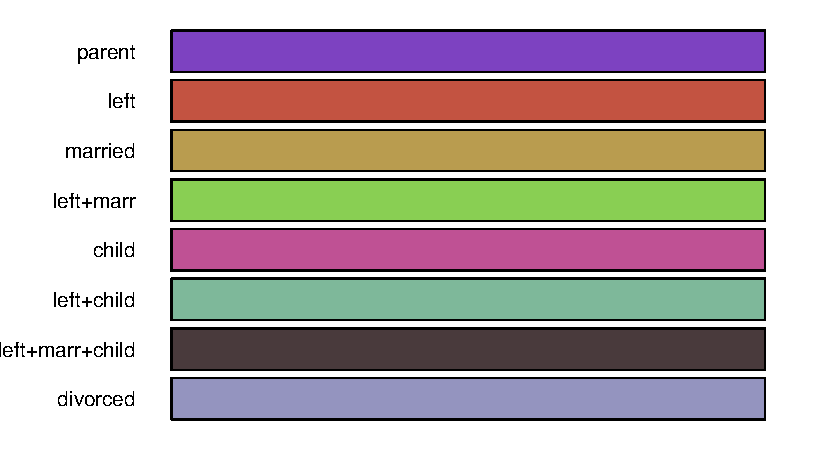
\includegraphics[width=\maxwidth]{figure/plotColors-1} \caption[Plotting colorpalettes can be handy when choosing colors for states]{Plotting colorpalettes can be handy when choosing colors for states.}\label{fig:plotColors}
\end{figure}


\end{knitrout}

The \texttt{ssplot}\index{ssplot@\texttt{ssplot}} function also accepts an object of class \texttt{hmm}. It can be used for plotting observations and/or most probable paths of hidden states or their state distributions. The function automatically computes the most probable paths of hidden states with the \texttt{hidden\_paths}\index{hiddenPaths@\texttt{hidden\_paths}} function, if the user does not provide them. Here the sequences are sorted according to multidimensional scaling scores that are computed from optimal matching dissimilarities for hidden state sequences. Any dissimilarity method available in \texttt{TraMineR} can be used instead of the default (see the documentation of the \texttt{seqdef} function for more information).

\begin{knitrout}
\definecolor{shadecolor}{rgb}{0.969, 0.969, 0.969}\color{fgcolor}\begin{kframe}
\begin{alltt}
\hlkwd{ssplot}\hlstd{(mc_fit}\hlopt{$}\hlstd{model,} \hlkwc{plots} \hlstd{=} \hlstr{"both"}\hlstd{,} \hlkwc{type} \hlstd{=} \hlstr{"I"}\hlstd{,} \hlkwc{sortv} \hlstd{=} \hlstr{"mds.hidden"}\hlstd{,}
  \hlkwc{xtlab} \hlstd{=} \hlnum{15}\hlopt{:}\hlnum{30}\hlstd{,} \hlkwc{xlab} \hlstd{=} \hlstr{"Age"}\hlstd{,} \hlkwc{title} \hlstd{=} \hlstr{"Observed and hidden state sequences"}\hlstd{)}
\end{alltt}
\end{kframe}\begin{figure}
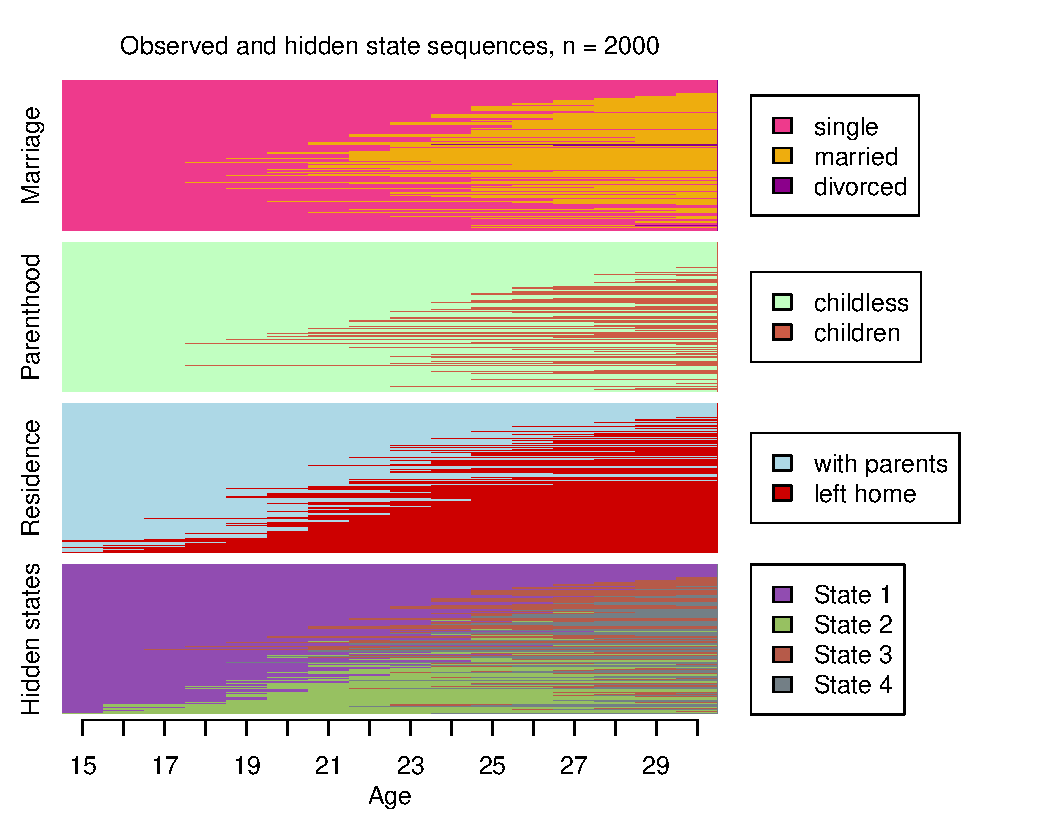
\includegraphics[width=\maxwidth]{figure/seqmppplot-1} \caption[Using the \texttt{ssplot} function to draw observations and the most probable hidden state paths given the model]{Using the \texttt{ssplot} function to draw observations and the most probable hidden state paths given the model.}\label{fig:seqmppplot}
\end{figure}


\end{knitrout}


\section{Mixture hidden Markov models}

Assume that we have a set of models (clusters) $\mathcal{M} = \{\mathcal{M}^1,\ldots, \mathcal{M}^K\}$, where $\mathcal{M}^k = \{\pi^k, A^k, B_1^k, \ldots, B_C^k\}$ for $k=1, \ldots, K$. For each subject $Y_i$, the prior cluster probability, i.e. the probability that  $Y_i$ is generated by submodel $\mathcal{M}^k$, is defined as multinomial distribution:
\begin{equation}
P(\mathcal{M}^k|\textbf{x}_i) = w_{ik}
= \frac{e^{\beta_k\textbf{x}_i}}{1 + \sum_{j=2}^K e^{\beta_j\textbf{x}_i}},
\end{equation}
where $\textbf{x}_i$ consists of the covariates relating to subject $Y_i$. The first cluster is set as the reference by fixing $\beta_1=0$. Note that by convention we use $\beta$ when referring to regression coefficients.

The mixture hidden Markov model (MHMM) can be regarded as a special type HMM by combining the $K$ submodels into one large hidden Markov model consisting of $\sum_{k=1}^K S_k$ states, where the initial state vector contains elements of form $w_k\pi^k$. Now the transition matrix is block diagonal
\begin{equation}
A =
 \begin{pmatrix}
  A^1   	& 0 			& \cdots & 0 			\\
  0 			& A^2 		& \cdots & 0 			\\
  \vdots  & \vdots  & \ddots & \vdots \\
  0 			& 0 			& \cdots & A^K
 \end{pmatrix},
\end{equation}
where the diagonal blocks $A^k, k=1,\ldots,K$, are square matrices containing the transition probabilities of one cluster. The off-diagonal blocks are zero matrices, so transitions between clusters are not allowed. Similarly, the emission matrices for each channel contains stacked emission matrices $B^k$.

The posterior cluster probabilities $P(M^k|Y_i, \textbf{x}_i)$ can be obtained as
\begin{equation}
  \begin{aligned}
P(M^k|Y_i, \textbf{x}_i) &= \frac{P(Y_i | M^k, \textbf{x}_i) P(M^k|\textbf{x}_i) }{P(Y_i| \textbf{x}_i)}\\
&= \frac{P(Y_i | M^k, \textbf{x}_i) P(M^k|\textbf{x}_i) }{\sum_{j=1}^K P(Y_i |M^j, \textbf{x}_i) P(M^j|\textbf{x}_i)} = \frac{L_k^i}{L^i},
  \end{aligned}
\end{equation}
where $L^i$ is the likelihood of the complete MHMM for individual $i$, and $L_k^i$ is the likelihood of cluster $k$ for individual $i$. These are straightforwardly computed from forward probabilities. Posterior cluster probabilities can be used e.g. for computing classification tables.

MHMMs are fitted in a similar way to HMMs using the \texttt{build\_mhmm}\index{buildmhmm@\texttt{build\_mhmm}} and \texttt{fit\_model}\index{fitmhmm@\texttt{fit\_model}} functions. Functions such as \texttt{logLik}\index{logLik@\texttt{logLik}}, \texttt{BIC}\index{BIC@\texttt{BIC}}, \texttt{trim\_model}\index{trimHMM@\texttt{trim\_model}}, and \texttt{mc\_to\_sc}\index{MCtoSC@\texttt{mc\_to\_sc}} work for \texttt{mhmm} objects as well.

Even though missing observations can be handled in sequences, the covariates must be completely observed for each subject. Subjects with missing covariates are easily dropped from the data set with the \texttt{complete.cases} function.

\begin{knitrout}
\definecolor{shadecolor}{rgb}{0.969, 0.969, 0.969}\color{fgcolor}\begin{kframe}
\begin{alltt}
\hlcom{# Starting values for initial state probabilities}
\hlstd{initial_probs1} \hlkwb{<-} \hlkwd{c}\hlstd{(}\hlnum{0.9}\hlstd{,} \hlnum{0.07}\hlstd{,} \hlnum{0.02}\hlstd{,} \hlnum{0.01}\hlstd{)}
\hlstd{initial_probs2} \hlkwb{<-} \hlkwd{c}\hlstd{(}\hlnum{0.9}\hlstd{,} \hlnum{0.04}\hlstd{,} \hlnum{0.03}\hlstd{,} \hlnum{0.01}\hlstd{,} \hlnum{0.01}\hlstd{,} \hlnum{0.01}\hlstd{)}

\hlcom{# Starting values for transition probabilities}
\hlstd{A1} \hlkwb{<-} \hlkwd{matrix}\hlstd{(}
  \hlkwd{c}\hlstd{(}\hlnum{0.80}\hlstd{,} \hlnum{0.16}\hlstd{,} \hlnum{0.03}\hlstd{,} \hlnum{0.01}\hlstd{,}
       \hlnum{0}\hlstd{,} \hlnum{0.90}\hlstd{,} \hlnum{0.07}\hlstd{,} \hlnum{0.03}\hlstd{,}
       \hlnum{0}\hlstd{,}    \hlnum{0}\hlstd{,} \hlnum{0.90}\hlstd{,}  \hlnum{0.1}\hlstd{,}
       \hlnum{0}\hlstd{,}    \hlnum{0}\hlstd{,}    \hlnum{0}\hlstd{,}    \hlnum{1}\hlstd{),}
  \hlkwc{nrow} \hlstd{=} \hlnum{4}\hlstd{,} \hlkwc{ncol} \hlstd{=} \hlnum{4}\hlstd{,} \hlkwc{byrow} \hlstd{=} \hlnum{TRUE}\hlstd{)}

\hlstd{A2} \hlkwb{<-} \hlkwd{matrix}\hlstd{(}
  \hlkwd{c}\hlstd{(}\hlnum{0.80}\hlstd{,} \hlnum{0.10}\hlstd{,} \hlnum{0.05}\hlstd{,} \hlnum{0.03}\hlstd{,} \hlnum{0.01}\hlstd{,} \hlnum{0.01}\hlstd{,}
       \hlnum{0}\hlstd{,} \hlnum{0.70}\hlstd{,} \hlnum{0.10}\hlstd{,} \hlnum{0.10}\hlstd{,} \hlnum{0.05}\hlstd{,} \hlnum{0.05}\hlstd{,}
       \hlnum{0}\hlstd{,}    \hlnum{0}\hlstd{,} \hlnum{0.85}\hlstd{,} \hlnum{0.01}\hlstd{,} \hlnum{0.10}\hlstd{,} \hlnum{0.04}\hlstd{,}
       \hlnum{0}\hlstd{,}    \hlnum{0}\hlstd{,}    \hlnum{0}\hlstd{,} \hlnum{0.90}\hlstd{,} \hlnum{0.05}\hlstd{,} \hlnum{0.05}\hlstd{,}
       \hlnum{0}\hlstd{,}    \hlnum{0}\hlstd{,}    \hlnum{0}\hlstd{,}    \hlnum{0}\hlstd{,} \hlnum{0.90}\hlstd{,}  \hlnum{0.1}\hlstd{,}
       \hlnum{0}\hlstd{,}    \hlnum{0}\hlstd{,}    \hlnum{0}\hlstd{,}    \hlnum{0}\hlstd{,}    \hlnum{0}\hlstd{,}    \hlnum{1}\hlstd{),}
  \hlkwc{nrow} \hlstd{=} \hlnum{6}\hlstd{,} \hlkwc{ncol} \hlstd{=} \hlnum{6}\hlstd{,} \hlkwc{byrow} \hlstd{=} \hlnum{TRUE}\hlstd{)}

\hlcom{# Starting values for emission probabilities}
\hlcom{# Cluster 1}
\hlkwd{alphabet}\hlstd{(child_seq)} \hlcom{# Checking for the order of observed states}
\end{alltt}
\begin{verbatim}
## [1] "childless" "children"
\end{verbatim}
\begin{alltt}
\hlstd{B1_child} \hlkwb{<-} \hlkwd{matrix}\hlstd{(}
  \hlkwd{c}\hlstd{(}\hlnum{0.99}\hlstd{,} \hlnum{0.01}\hlstd{,} \hlcom{# High probability for childless}
    \hlnum{0.99}\hlstd{,} \hlnum{0.01}\hlstd{,}
    \hlnum{0.99}\hlstd{,} \hlnum{0.01}\hlstd{,}
    \hlnum{0.99}\hlstd{,} \hlnum{0.01}\hlstd{),}
  \hlkwc{nrow} \hlstd{=} \hlnum{4}\hlstd{,} \hlkwc{ncol} \hlstd{=} \hlnum{2}\hlstd{,} \hlkwc{byrow} \hlstd{=} \hlnum{TRUE}\hlstd{)}

\hlkwd{alphabet}\hlstd{(marr_seq)}
\end{alltt}
\begin{verbatim}
## [1] "single"   "married"  "divorced"
\end{verbatim}
\begin{alltt}
\hlstd{B1_marr} \hlkwb{<-} \hlkwd{matrix}\hlstd{(}
  \hlkwd{c}\hlstd{(}\hlnum{0.98}\hlstd{,} \hlnum{0.01}\hlstd{,} \hlnum{0.01}\hlstd{,} \hlcom{# High probability for single}
    \hlnum{0.98}\hlstd{,} \hlnum{0.01}\hlstd{,} \hlnum{0.01}\hlstd{,}
    \hlnum{0.01}\hlstd{,} \hlnum{0.98}\hlstd{,} \hlnum{0.01}\hlstd{,} \hlcom{# High probability for married}
    \hlnum{0.01}\hlstd{,} \hlnum{0.01}\hlstd{,} \hlnum{0.98}\hlstd{),} \hlcom{# High probability for divorced}
  \hlkwc{nrow} \hlstd{=} \hlnum{4}\hlstd{,} \hlkwc{ncol} \hlstd{=} \hlnum{3}\hlstd{,} \hlkwc{byrow} \hlstd{=} \hlnum{TRUE}\hlstd{)}

\hlkwd{alphabet}\hlstd{(left_seq)}
\end{alltt}
\begin{verbatim}
## [1] "with parents" "left home"
\end{verbatim}
\begin{alltt}
\hlstd{B1_left} \hlkwb{<-} \hlkwd{matrix}\hlstd{(}
  \hlkwd{c}\hlstd{(}\hlnum{0.99}\hlstd{,} \hlnum{0.01}\hlstd{,} \hlcom{# High probability for living with parents}
    \hlnum{0.01}\hlstd{,} \hlnum{0.99}\hlstd{,} \hlcom{# High probability for having left home}
    \hlnum{0.01}\hlstd{,} \hlnum{0.99}\hlstd{,}
    \hlnum{0.01}\hlstd{,} \hlnum{0.99}\hlstd{),}
  \hlkwc{nrow} \hlstd{=} \hlnum{4}\hlstd{,} \hlkwc{ncol} \hlstd{=} \hlnum{2}\hlstd{,} \hlkwc{byrow} \hlstd{=} \hlnum{TRUE}\hlstd{)}

\hlcom{# Cluster 2}
\hlstd{B2_child} \hlkwb{<-} \hlkwd{matrix}\hlstd{(}
  \hlkwd{c}\hlstd{(}\hlnum{0.99}\hlstd{,} \hlnum{0.01}\hlstd{,} \hlcom{# High probability for childless}
    \hlnum{0.99}\hlstd{,} \hlnum{0.01}\hlstd{,}
    \hlnum{0.99}\hlstd{,} \hlnum{0.01}\hlstd{,}
    \hlnum{0.01}\hlstd{,} \hlnum{0.99}\hlstd{),}
  \hlkwc{nrow} \hlstd{=} \hlnum{4}\hlstd{,} \hlkwc{ncol} \hlstd{=} \hlnum{2}\hlstd{,} \hlkwc{byrow} \hlstd{=} \hlnum{TRUE}\hlstd{)}

\hlstd{B2_marr} \hlkwb{<-} \hlkwd{matrix}\hlstd{(}
  \hlkwd{c}\hlstd{(}\hlnum{0.98}\hlstd{,} \hlnum{0.01}\hlstd{,} \hlnum{0.01}\hlstd{,} \hlcom{# High probability for single}
    \hlnum{0.98}\hlstd{,} \hlnum{0.01}\hlstd{,} \hlnum{0.01}\hlstd{,}
    \hlnum{0.01}\hlstd{,} \hlnum{0.98}\hlstd{,} \hlnum{0.01}\hlstd{,} \hlcom{# High probability for married}
    \hlnum{0.01}\hlstd{,} \hlnum{0.70}\hlstd{,} \hlnum{0.29}\hlstd{),}
  \hlkwc{nrow} \hlstd{=} \hlnum{4}\hlstd{,} \hlkwc{ncol} \hlstd{=} \hlnum{3}\hlstd{,} \hlkwc{byrow} \hlstd{=} \hlnum{TRUE}\hlstd{)}

\hlstd{B2_left} \hlkwb{<-} \hlkwd{matrix}\hlstd{(}
  \hlkwd{c}\hlstd{(}\hlnum{0.99}\hlstd{,} \hlnum{0.01}\hlstd{,} \hlcom{# High probability for living with parents}
    \hlnum{0.01}\hlstd{,} \hlnum{0.99}\hlstd{,} \hlcom{# High probability for having left home}
    \hlnum{0.01}\hlstd{,} \hlnum{0.99}\hlstd{,}
    \hlnum{0.01}\hlstd{,} \hlnum{0.99}\hlstd{),}
  \hlkwc{nrow} \hlstd{=} \hlnum{4}\hlstd{,} \hlkwc{ncol} \hlstd{=} \hlnum{2}\hlstd{,} \hlkwc{byrow} \hlstd{=} \hlnum{TRUE}\hlstd{)}

\hlcom{# Cluster 3}
\hlstd{B3_child} \hlkwb{<-} \hlkwd{matrix}\hlstd{(}
  \hlkwd{c}\hlstd{(}\hlnum{0.99}\hlstd{,} \hlnum{0.01}\hlstd{,} \hlcom{# High probability for childless}
    \hlnum{0.99}\hlstd{,} \hlnum{0.01}\hlstd{,}
    \hlnum{0.01}\hlstd{,} \hlnum{0.99}\hlstd{,}
    \hlnum{0.99}\hlstd{,} \hlnum{0.01}\hlstd{,}
    \hlnum{0.01}\hlstd{,} \hlnum{0.99}\hlstd{,}
    \hlnum{0.01}\hlstd{,} \hlnum{0.99}\hlstd{),}
  \hlkwc{nrow} \hlstd{=} \hlnum{6}\hlstd{,} \hlkwc{ncol} \hlstd{=} \hlnum{2}\hlstd{,} \hlkwc{byrow} \hlstd{=} \hlnum{TRUE}\hlstd{)}

\hlstd{B3_marr} \hlkwb{<-} \hlkwd{matrix}\hlstd{(}
  \hlkwd{c}\hlstd{(}\hlnum{0.98}\hlstd{,} \hlnum{0.01}\hlstd{,} \hlnum{0.01}\hlstd{,} \hlcom{# High probability for single}
    \hlnum{0.98}\hlstd{,} \hlnum{0.01}\hlstd{,} \hlnum{0.01}\hlstd{,}
    \hlnum{0.98}\hlstd{,} \hlnum{0.01}\hlstd{,} \hlnum{0.01}\hlstd{,}
    \hlnum{0.01}\hlstd{,} \hlnum{0.98}\hlstd{,} \hlnum{0.01}\hlstd{,} \hlcom{# High probability for married}
    \hlnum{0.01}\hlstd{,} \hlnum{0.98}\hlstd{,} \hlnum{0.01}\hlstd{,}
    \hlnum{0.01}\hlstd{,} \hlnum{0.01}\hlstd{,} \hlnum{0.98}\hlstd{),} \hlcom{# High probability for divorced}
  \hlkwc{nrow} \hlstd{=} \hlnum{6}\hlstd{,} \hlkwc{ncol} \hlstd{=} \hlnum{3}\hlstd{,} \hlkwc{byrow} \hlstd{=} \hlnum{TRUE}\hlstd{)}

\hlstd{B3_left} \hlkwb{<-} \hlkwd{matrix}\hlstd{(}
  \hlkwd{c}\hlstd{(}\hlnum{0.99}\hlstd{,} \hlnum{0.01}\hlstd{,} \hlcom{# High probability for living with parents}
    \hlnum{0.01}\hlstd{,} \hlnum{0.99}\hlstd{,}
    \hlnum{0.50}\hlstd{,} \hlnum{0.50}\hlstd{,}
    \hlnum{0.01}\hlstd{,} \hlnum{0.99}\hlstd{,}
    \hlnum{0.01}\hlstd{,} \hlnum{0.99}\hlstd{,}
    \hlnum{0.01}\hlstd{,} \hlnum{0.99}\hlstd{),}
  \hlkwc{nrow} \hlstd{=} \hlnum{6}\hlstd{,} \hlkwc{ncol} \hlstd{=} \hlnum{2}\hlstd{,} \hlkwc{byrow} \hlstd{=} \hlnum{TRUE}\hlstd{)}

\hlcom{# Birth cohort}
\hlstd{biofam3c}\hlopt{$}\hlstd{covariates}\hlopt{$}\hlstd{cohort} \hlkwb{<-} \hlkwd{cut}\hlstd{(}
  \hlstd{biofam3c}\hlopt{$}\hlstd{covariates}\hlopt{$}\hlstd{birthyr,} \hlkwd{c}\hlstd{(}\hlnum{1908}\hlstd{,} \hlnum{1935}\hlstd{,} \hlnum{1945}\hlstd{,} \hlnum{1957}\hlstd{))}
\hlstd{biofam3c}\hlopt{$}\hlstd{covariates}\hlopt{$}\hlstd{cohort} \hlkwb{<-} \hlkwd{factor}\hlstd{(}
  \hlstd{biofam3c}\hlopt{$}\hlstd{covariates}\hlopt{$}\hlstd{cohort,}
  \hlkwc{labels} \hlstd{=} \hlkwd{c}\hlstd{(}\hlstr{"1909-1935"}\hlstd{,} \hlstr{"1936-1945"}\hlstd{,} \hlstr{"1946-1957"}\hlstd{))}

\hlcom{# Build MHMM}
\hlstd{init_mhmm} \hlkwb{<-} \hlkwd{build_mhmm}\hlstd{(}
  \hlkwc{observations} \hlstd{=} \hlkwd{list}\hlstd{(marr_seq, child_seq, left_seq),}
  \hlkwc{transition_probs} \hlstd{=} \hlkwd{list}\hlstd{(A1, A1, A2),}
  \hlkwc{emission_probs} \hlstd{=} \hlkwd{list}\hlstd{(}\hlkwd{list}\hlstd{(B1_marr, B1_child, B1_left),}
                        \hlkwd{list}\hlstd{(B2_marr, B2_child, B2_left),}
                        \hlkwd{list}\hlstd{(B3_marr, B3_child, B3_left)),}
  \hlkwc{initial_probs} \hlstd{=} \hlkwd{list}\hlstd{(initial_probs1, initial_probs1, initial_probs2),}
  \hlkwc{formula} \hlstd{=} \hlopt{~}\hlstd{sex} \hlopt{+} \hlstd{cohort,} \hlkwc{data} \hlstd{= biofam3c}\hlopt{$}\hlstd{covariates,}
  \hlkwc{cluster_names} \hlstd{=} \hlkwd{c}\hlstd{(}\hlstr{"Cluster 1"}\hlstd{,} \hlstr{"Cluster 2"}\hlstd{,} \hlstr{"Cluster 3"}\hlstd{),}
  \hlkwc{channel_names} \hlstd{=} \hlkwd{c}\hlstd{(}\hlstr{"Marriage"}\hlstd{,} \hlstr{"Parenthood"}\hlstd{,} \hlstr{"Residence"}\hlstd{))}

\hlkwd{set.seed}\hlstd{(}\hlnum{456}\hlstd{)}
\hlstd{fit_mhmm} \hlkwb{<-} \hlkwd{fit_model}\hlstd{(}
  \hlstd{init_mhmm,} \hlkwc{threads} \hlstd{=} \hlnum{4}\hlstd{,} \hlkwc{control_em} \hlstd{=}
    \hlkwd{list}\hlstd{(}\hlkwc{restart} \hlstd{=} \hlkwd{list}\hlstd{(}\hlkwc{times} \hlstd{=} \hlnum{50}\hlstd{,} \hlkwc{transition} \hlstd{=} \hlnum{FALSE}\hlstd{)))}
\end{alltt}
\end{kframe}
\end{knitrout}

The \texttt{summary}\index{summaryMHMM@\texttt{summary.mhmm}} method computes summaries of the MHMM, e.g. standard errors for covariates and prior and posterior probabilities for subjects. A \texttt{print}\index{printSummaryMHMM@\texttt{print.summary.mhmm}} method shows some summaries of these: estimates and standard errors for covariates, log-likelihood and BIC, and information on most probable clusters and prior probabilities. Parameter estimates for transitions, emissions, and initial probabilities are omitted by default.

There are two types of standard errors which can be computed for regression coefficients. The conditional standard errors can be computed using analytical formulas for Hessian, but these do not take account the estimation uncertainty regarding the other model parameters. For unconditional standard errors which take account of possible correlation between the estimates of $\beta$ and other model parameters, the Hessian is computed using finite difference approximation of the Jacobian of the analytical gradients. Naturally, the latter option is computationally more demanding, but it should still be a preferred option in final analysis as it gives more realistic results.

\begin{knitrout}
\definecolor{shadecolor}{rgb}{0.969, 0.969, 0.969}\color{fgcolor}\begin{kframe}
\begin{alltt}
\hlkwd{summary}\hlstd{(fit_mhmm}\hlopt{$}\hlstd{model,} \hlkwc{conditional_se} \hlstd{=} \hlnum{FALSE}\hlstd{)}
\end{alltt}
\begin{verbatim}
## Covariate effects :
## Cluster 1 is the reference.
## 
## Cluster 2 :
##                  Estimate  Std. error
## (Intercept)        1.1939       0.204
## sexwoman          -0.0744       0.162
## cohort1936-1945    0.1467       0.216
## cohort1946-1957   -0.0230       0.218
## 
## Cluster 3 :
##                  Estimate  Std. error
## (Intercept)         0.258       0.208
## sexwoman            0.253       0.185
## cohort1936-1945    -0.557       0.234
## cohort1946-1957    -1.106       0.228
## 
## Log-likelihood: -12654.53   BIC: 26367.16 
## 
## Means of prior cluster probabilities :
## Cluster 1 Cluster 2 Cluster 3 
##     0.197     0.642     0.161 
## 
## Most probable clusters :
##             Cluster 1  Cluster 2  Cluster 3
## count             313       1412        275
## proportion      0.156      0.706      0.138
## 
## Classification table :
## Mean cluster probabilities (in columns) by the most probable cluster (rows)
## 
##           Cluster 1 Cluster 2 Cluster 3
## Cluster 1  8.39e-01   0.16148  9.90e-08
## Cluster 2  9.28e-02   0.87280  3.44e-02
## Cluster 3  6.46e-05   0.00452  9.95e-01
\end{verbatim}
\end{kframe}
\end{knitrout}

The classification table shows the mean probabilities of belonging to each cluster by the most probable cluster. The most probable cluster is determined by the posterior cluster probabilities. A good model shoud have high proportions in the diagonal. Here, for individuals assigned to cluster 1, the average probability for cluster 1 is 0.84, 0.16 for cluster 2, and close to 0 for cluster 3. The highest probability for the assigned cluster is 0.93 for cluster 3.

It is possible to convert a \texttt{mhmm} object into a list of separate \texttt{hmm} objects with the \texttt{separate\_mhmm}\index{sepMixHMM@\texttt{separate\_mhmm}} function. These can then be plotted with functions designed for \texttt{hmm} class objects, e.g. \texttt{ssp}\index{ssp@\texttt{ssp}} and \texttt{gridplot}\index{gridplot@\texttt{gridplot}}. However, usually an easier option is to use plotting functions and methods designed for \texttt{mhmm} objects.


\section{Plotting mixture hidden Markov models}

Also MHMMs are plotted with the \texttt{plot}\index{plot.mhmm@\texttt{plot.mhmm}} method. The user can choose between an interactive mode (\texttt{interactive=TRUE}), where the model for each cluster is plotted separately, and a combined plot with all models in one plot. The clusters are determined according to the \texttt{posterior\_probs}\index{posteriorProbs@\texttt{posterior\_probs}} function, which is called automatically. Clusters with no subjects get removed from the plot, and the function gives a warning. With the \texttt{which.plots} argument the user can choose which clusters to plot.

\begin{knitrout}
\definecolor{shadecolor}{rgb}{0.969, 0.969, 0.969}\color{fgcolor}\begin{kframe}
\begin{alltt}
\hlkwd{plot}\hlstd{(fit_mhmm}\hlopt{$}\hlstd{model,} \hlkwc{interactive} \hlstd{=} \hlnum{FALSE}\hlstd{,} \hlkwc{which.plots} \hlstd{=} \hlnum{2}\hlopt{:}\hlnum{3}\hlstd{,} \hlkwc{nrow} \hlstd{=} \hlnum{2}\hlstd{,}
  \hlkwc{legend.prop} \hlstd{=} \hlnum{0.35}\hlstd{,} \hlkwc{cex.legend} \hlstd{=} \hlnum{1.5}\hlstd{,} \hlkwc{edge.label.cex} \hlstd{=} \hlnum{1.5}\hlstd{,}
  \hlkwc{ncol.legend} \hlstd{=} \hlnum{2}\hlstd{)}
\end{alltt}
\end{kframe}
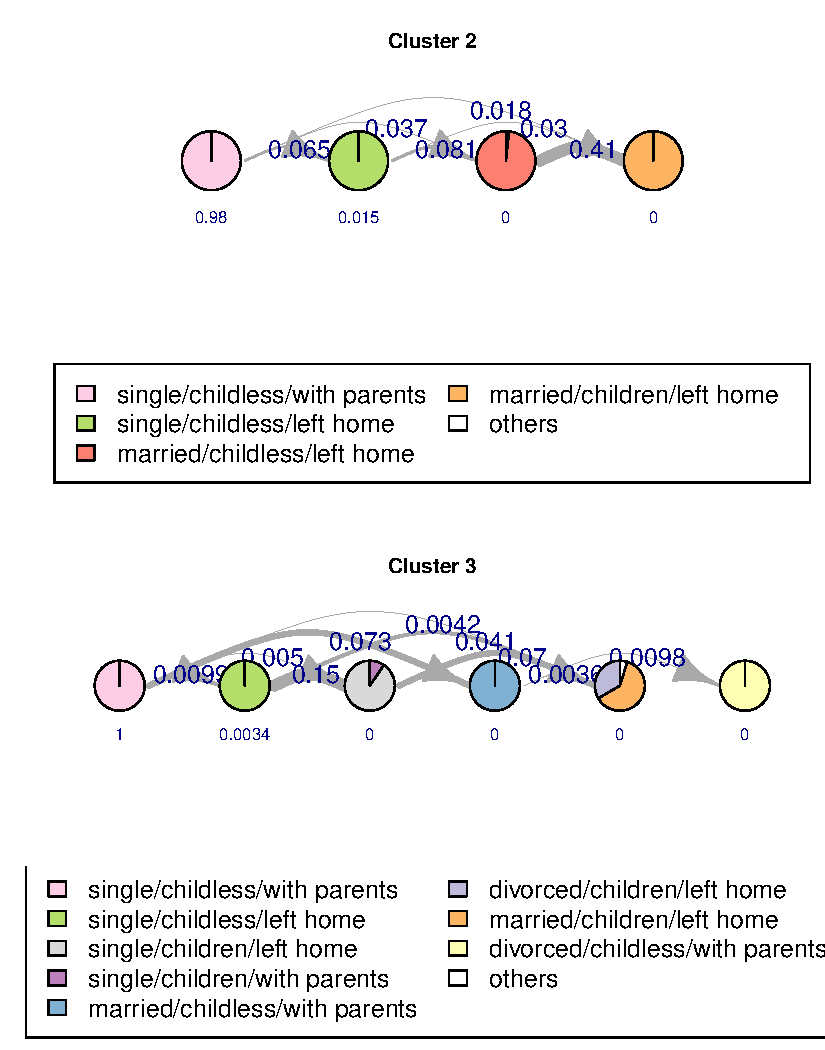
\includegraphics[width=\maxwidth]{figure/MHMMplot-1} 

\end{knitrout}

The equivalent to the \texttt{ssplot} function for MHMMs is called \texttt{mssplot}\index{mssplot@\texttt{mssplot}}. It plots stacked sequence plots separately for each (chosen) cluster. If the user asks to plot more than one cluster, the function is interactive by default. If \texttt{ask = TRUE}, the cluster plots are chosen one by one by selecting their numbers from the menu; otherwise they are plotted in the order they appear in the \texttt{mhmm} object.

\begin{knitrout}
\definecolor{shadecolor}{rgb}{0.969, 0.969, 0.969}\color{fgcolor}\begin{kframe}
\begin{alltt}
\hlkwd{mssplot}\hlstd{(fit_mhmm}\hlopt{$}\hlstd{model,} \hlkwc{plots} \hlstd{=} \hlstr{"both"}\hlstd{,} \hlkwc{ask} \hlstd{=} \hlnum{FALSE}\hlstd{,} \hlkwc{which.plots} \hlstd{=} \hlnum{1}\hlstd{)}
\end{alltt}
\end{kframe}
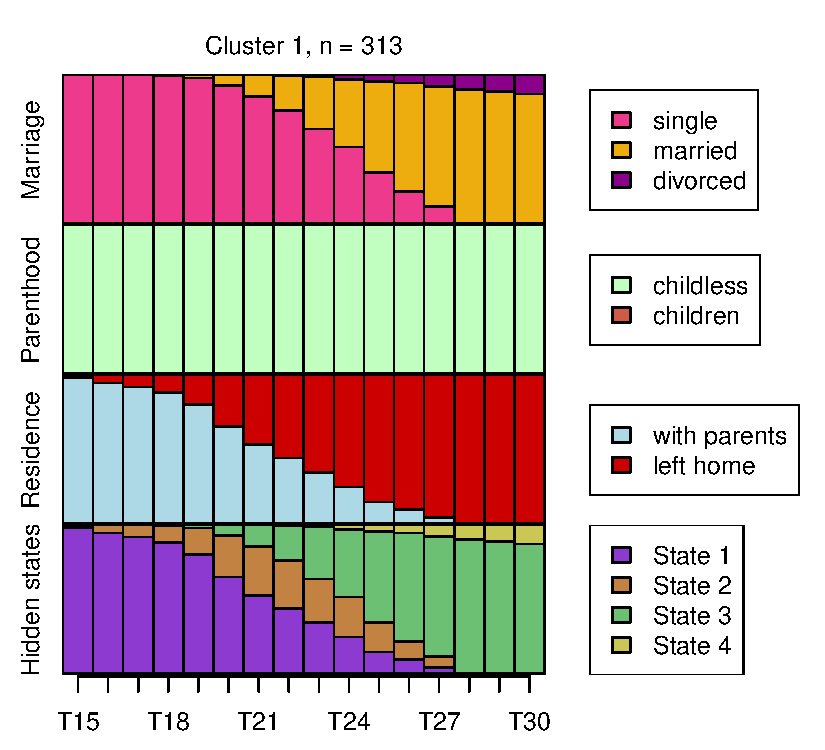
\includegraphics[width=\maxwidth]{figure/MHMMssplot-1} 

\end{knitrout}


\newpage
\bibliographystyle{newapa}
\bibliography{Art12}
\printindex

\end{document}
